%--------------------------------------------------------------------------------------%--------------------------------------------------------------------------------------
%
%  Global settings, dont change it! (excapt additional \usepackage commands)
%  Always use PDFLatex!
%
%--------------------------------------------------------------------------------------%--------------------------------------------------------------------------------------
\documentclass[a4paper, 12pt, oneside, openany, BCOR1cm,toc=chapterentrywithdots]{scrbook}

\usepackage{graphicx}           % use for pdfLatex
\usepackage{makeidx} % f\"{u}r Benutzung des Befehls \printindex
\usepackage[colorlinks=false]{hyperref}
\usepackage{tocbibind}
\usepackage{blindtext}
\usepackage{subfigure}
\usepackage{acronym}
\usepackage[table]{xcolor}
\usepackage{pifont}
\newcommand{\cmark}{\textcolor{green!45!black}{\ding{51}}}
\newcommand{\xmark}{\textcolor{red!60!black}{\ding{55}}}

\hypersetup{%
bookmarksnumbered=true, hyperindex=true,
%
%Im Acrobat Reader Subtitel 1. Ebene anzeigen
bookmarksopen=true, bookmarksopenlevel=1,
%
pdfborder=0 0 0 % Keine Box um die Links!
}

% --------------------------------------------------------------
% Force Tables and List to be added in Table of Content
% --------------------------------------------------------------

\renewcommand*{\tableofcontents}{%
  	\begingroup
  	\tocsection
  	\tocfile{\contentsname}{toc}
  	\endgroup
}
\renewcommand*{\listoffigures}{%
  	\begingroup
  	\tocsection
  	\tocfile{\listfigurename}{lof}
  	\endgroup
}
\renewcommand{\listoftables}{
	\begingroup
	\tocsection
	\tocfile{\listtablename}{lot}
	\endgroup
}
\begin{document}

%--------------------------------------------------------------------------------------%--------------------------------------------------------------------------------------
%
%  Here starts the userspace !
%
%--------------------------------------------------------------------------------------%--------------------------------------------------------------------------------------

%--------titlepage
\begin{titlepage}

{
    \begin{center}
        \raisebox{-1ex}{\includegraphics[scale=1.5]
        %{TU_Chemnitz_positiv_gruen.pdf}}\\
    \end{center}
    \vspace{0.5cm}
}

\begin{center}

\LARGE{\textbf{Recommendation System for ASPICE (SWE1-SWE6) Process Assessment}}\\
\vspace{1cm}


\Large{\textbf{Master Thesis}}\\
\vspace{1cm}
Submitted in Fulfilment of the\\
Requirements for the Academic Degree\\
M.Sc. Automotive Software Engineering\\
\vspace{0.5cm}
Dept. of Computer Science\\
Chair of Computer Engineering
\end{center}
\vspace{2cm}
Submitted by: Faizan Ahmed\\
Student ID: \\
Date: 17.09.2026\\
\vspace{0.3cm}\\
%Supervising tutor: Prof. Dr. W. Hardt \\
(further supervisors)

\end{titlepage}

%---------------------------------------------------------
% Abstract
%---------------------------------------------------------

\addchap*{Abstract}
\blindtext
\\\\
\textbf{Keywords: ASPICE, Recommender Systems, Contextual Multi-Armed Bandit, LinUCB, Process Assessment}

%---------------------------------------------------------
% Table of Contents, List of figures, List of Tables
%---------------------------------------------------------

\tableofcontents
\listoffigures
\listoftables

%---------------------------------------------------------
% List of Abbreviations
%---------------------------------------------------------
\twocolumn
\addchap{List of Abbreviations}
\begin{acronym}[HTTPS]
 \acro{ASPICE}{Automotive Software Process Improvement and Capability dEtermination}
 \acro{SPICE}{Software Process Improvement and Capability dEtermination}
 \acro{PRM}{Process Reference Model}
 \acro{PAM}{Process Assessment Model}
 \acro{BP}{Base Practice}
 \acro{SWE}{Software Engineering (process group)}
 \acro{MAB}{Multi-Armed Bandit}
 \acro{CMAB}{Contextual Multi-Armed Bandit}
 \acro{UCB}{Upper Confidence Bound}
 \acro{LinUCB}{Linear Upper Confidence Bound}
 \acro{RL}{Reinforcement Learning}
 \acro{ER}{Entity-Relationship}
 \acro{CRUD}{Create, Read, Update, Delete}
 \acro{ORM}{Object-Relational Mapping}
 \acro{API}{Application Programming Interface}
 \acro{REST}{Representational State Transfer}
 \acro{JWT}{JSON Web Token}
 \acro{JSON}{JavaScript Object Notation}
 \acro{SQL}{Structured Query Language}
 \acro{DB}{Database}
 \acro{UI}{User Interface}
 \acro{UX}{User Experience}
 \acro{HTTP}{Hypertext Transfer Protocol}
 \acro{HTTPS}{Hypertext Transfer Protocol Secure}
 \acro{TLS}{Transport Layer Security}
\end{acronym}

\onecolumn
%---------------------------------------------------------
% Here starts the real work
%---------------------------------------------------------

\chapter{Introduction}
\label{chap:introduction}
% \input{src/introduction}

This chapter lays out the context and the core problem behind this research, along with the
main objectives of the thesis. It begins with the problem statement and motivation that bring
focus on the need for continuous, ASPICE-aligned process assessment in automotive software
development, followed by the research questions, the contributions of this work, and its scope,
and ends with an overview of the structure of the thesis.

\section{Problem Statement}

Automotive Software Process Improvement and Capability dEtermination (ASPICE) is a process
assessment model that automotive OEMs and suppliers use to judge how well a supplier's software
development process is being carried out~\cite{vdaqmc2023pam}. It does not assess the software
itself, but the process behind it: whether requirements are properly analyzed, whether the
architecture and detailed design stay consistent with those requirements, and whether the
resulting software is properly verified. For the Software Engineering process group,
SWE.1 through SWE.6, this means checking every step from initial requirements analysis to final
software verification.

In practice, this checking is carried out through structured audits. A certified assessor visits
a project at defined milestones, reviews the available evidence, and rates each process against
a fixed scale, from \emph{not achieved} to \emph{fully achieved}~\cite{vdaqmc2023pam,murphy_aspice_0to60}.
This works well as a snapshot of process capability at a single point in time, but it says little
about what happens between audits.

This is where the core problem of this thesis lies. Once a project has been assessed, there is no
continuous way to check whether its processes are still being followed correctly. A weakness
introduced shortly after an audit, in a requirement that is poorly analyzed or a design decision
that is never properly reviewed, can go unnoticed for months, until it either resurfaces in the
next scheduled audit or shows up later as a defect~\cite{datsogiannis2024early}. By that point,
fixing it costs far more than it would have if it had been caught
early~\cite{schauffele2016automotive,jiang2013earlylifecycle}. ASPICE, as it is normally applied,
is simply not built to close this gap: it produces a rating at audit time, not a signal a
development team can act on in between.

This thesis takes that gap as its starting point: \emph{can the SWE.1--SWE.6 base practices be
turned into something stakeholders check continuously, as part of daily development, rather than
only when an assessor is on site?}

\section{Motivation}

The motivation for this thesis comes from a practical challenge in modern automotive software
development. Vehicles are becoming increasingly software-driven and connected, with complex
in-vehicle systems, cloud services, and software that must remain compatible across different
generations of platforms~\cite{zhang2021canbus,furst2010challenges}. As this complexity grows,
process weaknesses can become harder to detect and more costly to address when they are
discovered late. This makes regular and effective process assessment increasingly important.

Automotive SPICE (ASPICE) provides a well-established framework for assessing software
development processes. However, traditional assessment is mainly carried out through structured,
periodic audits. In most cases, this means that stakeholders are asked a large number of
predefined questions, even though not every question is equally useful in every situation. Some
questions may provide little additional information, while another question, asked at the right
moment, could reveal a significant weakness. This leads to an important question: \emph{can the
same assessment value be achieved by asking fewer, but more relevant, questions?}

This idea is supported by research on reinforcement-learning-based recommender systems, which
shows that a system can learn to select questions that are more useful for the situation rather
than simply following a fixed sequence~\cite{datsogiannis2024early}. The same principle is
promising for ASPICE assessment. The value of a question can change depending on what has
already been covered, which process areas appear weak, the capability level being explored, and
the role of the stakeholder providing the answer. A contextual multi-armed bandit (CMAB) is
therefore a suitable approach because it can use this changing context to decide which question
should be asked next.

Previous research has already explored ASPICE-derived questions selected through a CMAB approach
and has compared different bandit algorithms in simulated
settings~\cite{datsogiannis2024early,datsogiannis2025recommender}. However, an important step is
still missing: moving from a promising concept demonstrated through simulation to a working
system evaluated with real assessment data. This gap is the main motivation for this thesis.

The thesis therefore develops a web application that adaptively selects questions from the
SWE.1--SWE.6 process group based on the information available during an assessment session. The
responses are then used to identify and classify potential process weaknesses. The purpose is
not to replace expert judgement or the principles of ASPICE. Rather, it is to make the assessment
process more focused by helping the system ask the \emph{right question at the right time}.

Ultimately, this research is motivated by the possibility of making process assessment less
dependent on lengthy, fixed questionnaires and more responsive to the situation being assessed.
By implementing the approach as a working web application and evaluating it with real audit
sessions, rather than simulated data alone, this thesis aims to show that adaptive question
selection can make ASPICE assessment both practical to use and continuous over time.

\section{Research Questions}

This thesis is guided by four research questions:

\begin{itemize}
  \item \textbf{RQ1.} How can the base practices of ASPICE SWE.1--SWE.6 be transformed into a
  structured, weighted question bank of auditor-style questions, mapped to SWE processes and
  stakeholder roles?
  \item \textbf{RQ2.} How can a web-based recommendation system select a small number of
  well-targeted questions per evaluation cycle, rather than working through the entire question
  bank?
  \item \textbf{RQ3.} How can stakeholder answers be classified automatically into a process
  weakness rating for each SWE process, without requiring a human assessor's judgement?
  \item \textbf{RQ4.} How can these results be presented so that process weaknesses, and how
  they change across software releases, are visible early, rather than only at the next
  scheduled ASPICE audit?
\end{itemize}

\section{Contributions}

This thesis makes the following contributions, matched to the research questions above:

\begin{itemize}
  \item \textbf{RQ1.} A structured ASPICE SWE.1--SWE.6 question bank in which every question is
  traceable to a specific base practice and carries stakeholder-role assignments and weighted
  answer options.
  \item \textbf{RQ2.} A CMAB-based recommendation engine, using the LinUCB algorithm, that
  selects a small number of well-targeted questions per session from a session-state context
  covering stakeholder role, progress, and process and capability-level coverage so far.
  \item \textbf{RQ3.} A rule-based weakness classifier that scores every assessed (process,
  capability level) cell and ranks the resulting weaknesses automatically, without requiring a
  labelled training dataset or a human assessor's judgement.
  \item \textbf{RQ4.} A results dashboard that presents weakness classifications per SWE process
  and their trends across sessions, giving early visibility instead of waiting for the next
  scheduled audit.
  \item A full web application, built on FastAPI, React, and PostgreSQL, that ties the four
  contributions above together end to end for real users.
  \item An evaluation on real, non-simulated pilot sessions. Both supervisor
  papers~\cite{datsogiannis2024early,datsogiannis2025recommender} defer that evaluation to
  future work; this thesis provides it for the SWE.1--SWE.6 scope.
\end{itemize}

\section{Scope and Limitations}

This thesis focuses on one part of ASPICE: the Software Engineering process group, SWE.1 through
SWE.6, and capability levels L1 to L3 (Performed, Managed, Established). System Engineering,
Validation, Management, Supporting, and Process Improvement are not covered, and neither are
capability levels L4 and L5. Those higher levels are about quantitative process control and
organization-wide improvement, which need evidence collected across many projects over time
rather than what a single stakeholder can report in one session.

This narrower scope brings two limitations that are worth stating clearly.

\begin{itemize}
  \item Capability levels L2 and L3 partly depend on how a process is defined and deployed
  across an organization, not just how it is performed on one project~\cite{vdaqmc2023pam}. A
  session answered by a single stakeholder can only approximate this from that person's point of
  view; it is not a substitute for an assessor examining the organization's actual process
  assets.
  \item The weights given to answer options in this thesis were not checked by an independent
  panel of experts. Dimitrios validated these question weights through interviews with
  automotive experts~\cite{datsogiannis2024early}; doing the same here is left for future work.
\end{itemize}

\section{Structure of the Thesis}

Chapter~\ref{chap:background} introduces ASPICE, recommender systems, and multi-armed bandits,
enough to follow everything that comes after. Chapter~\ref{chap:sota} places this thesis next to
the two supervisor papers discussed above, and against how ASPICE is normally practiced.
Chapter~\ref{chap:architecture} explains how the system is built: the database schema, the CMAB
engine, the weakness classifier, and the API and frontend design. Chapter~\ref{chap:implementation}
covers how that design was actually implemented. Chapter~\ref{chap:methodology} explains how the
system was evaluated, and Chapter~\ref{chap:results} presents what that evaluation found.
Chapter~\ref{chap:conclusion} closes the thesis by returning to the research questions and
discussing what is left for future work.

\chapter{Background and Fundamentals}
\label{chap:background}
% \input{src/background}

This chapter introduces the three ideas the rest of the thesis builds on: what ASPICE is and how
it is normally carried out, what a recommender system does in general, and what a multi-armed
bandit is. Readers already familiar with any of these can skip ahead; Chapter~\ref{chap:architecture}
assumes the vocabulary introduced here.

\section{Automotive SPICE (ASPICE)}

Automotive SPICE (ASPICE) is a process assessment model that automotive OEMs and suppliers use
to check how well a supplier develops software and systems~\cite{vdaqmc2023pam}. It does not
assess the product itself; it assesses the process used to build the product. A supplier is
rated not on whether its software works, but on whether its development process reliably
produces evidence that requirements were captured, designed against, built, and
verified~\cite{vdaqmc2023pam,murphy_aspice_0to60}.

\subsection{Process Reference and Assessment Models (PRM/PAM)}

ASPICE is built from two related models. The Process Reference Model (PRM) lists the processes
a supplier can be assessed against, along with a purpose and a set of expected outcomes for
each one. The Process Assessment Model (PAM) adds the machinery needed to actually rate those
processes: a set of capability levels, and indicators, called base practices and generic
practices, that an assessor looks for as evidence~\cite{vdaqmc2023pam}. Put together, this gives
a two-dimensional picture of process capability: a \emph{process dimension} (which process is
being looked at) and a \emph{capability dimension} (how well it is being carried out). ASPICE's
own measurement framework, which defines the capability dimension, is an adaptation of the
international standard for process assessment,
ISO/IEC~33020~\cite{iso33020_2019,vdaqmc2023pam}, and its core terms, such as
\emph{information item} and \emph{process attribute}, come from
ISO/IEC~33001~\cite{iso33001_2015}.

Figure~\ref{fig:aspice-model} shows the full process reference model maintained by the VDA
Quality Management Center, the organization behind the ASPICE
standard~\cite{vdaqmc_website,vdaqmc2023pam}. The processes are colour-coded into three
life-cycle categories and further split into process groups, each identified by a two-letter
code.

\begin{figure}[h]
  \centering
  
\includegraphics[width=\textwidth]{src/aspice_model.png}
  \caption{The Automotive SPICE process reference model, with the Software Engineering process
  group (SWE) highlighted in red. Reproduced from the official process reference model published
  by the VDA Quality Management Center~\cite{vdaqmc_website,vdaqmc2023pam}.}
  \label{fig:aspice-model}
\end{figure}

\begin{description}
  \item[Acquisition (ACQ)] Tracks the performance of an external, contracted supplier.
  \item[Supply (SPL)] Controls how a finished product is released to a customer.
  \item[System Engineering (SYS)] Takes stakeholder needs through system-level requirements,
  architecture, integration, and verification.
  \item[Software Engineering (SWE)] Does the same at the software level, from requirements to
  verification; this is the group this thesis works with.
  \item[Hardware Engineering (HWE)] Mirrors SWE for hardware components.
  \item[Machine Learning Engineering (MLE)] Covers requirements, architecture, training, and
  testing specific to machine-learning components.
  \item[Validation (VAL)] Checks that the finished product meets real-world stakeholder
  expectations, not just the written requirements.
  \item[Supporting Process (SUP)] Covers quality assurance, configuration management, problem
  resolution management, change request management, and machine-learning data management.
  \item[Management (MAN)] Covers project management, risk management, and measurement.
  \item[Process Improvement (PIM)] Covers how the organization improves its own processes over
  time.
  \item[Reuse (REU)] Covers managing products developed for reuse across projects.
\end{description}

This grouping lets a supplier be assessed only on the process groups relevant to what it
actually builds. This thesis works entirely within one primary life-cycle group: Software
Engineering (SWE).

\subsection{The SWE Process Group: SWE.1--SWE.6}

The Software Engineering process group covers everything from writing software requirements to
verifying the finished software. It contains six processes, described below.

Figure~\ref{fig:v-model} shows how the six processes fit into the V-model used across automotive
software development~\cite{vmodel_visure}. Requirements and design work run down the left side,
and the corresponding verification and test work runs back up the right side, so each process on
the left has a matching process on the right that checks its output.

\begin{figure}[h]
  \centering
  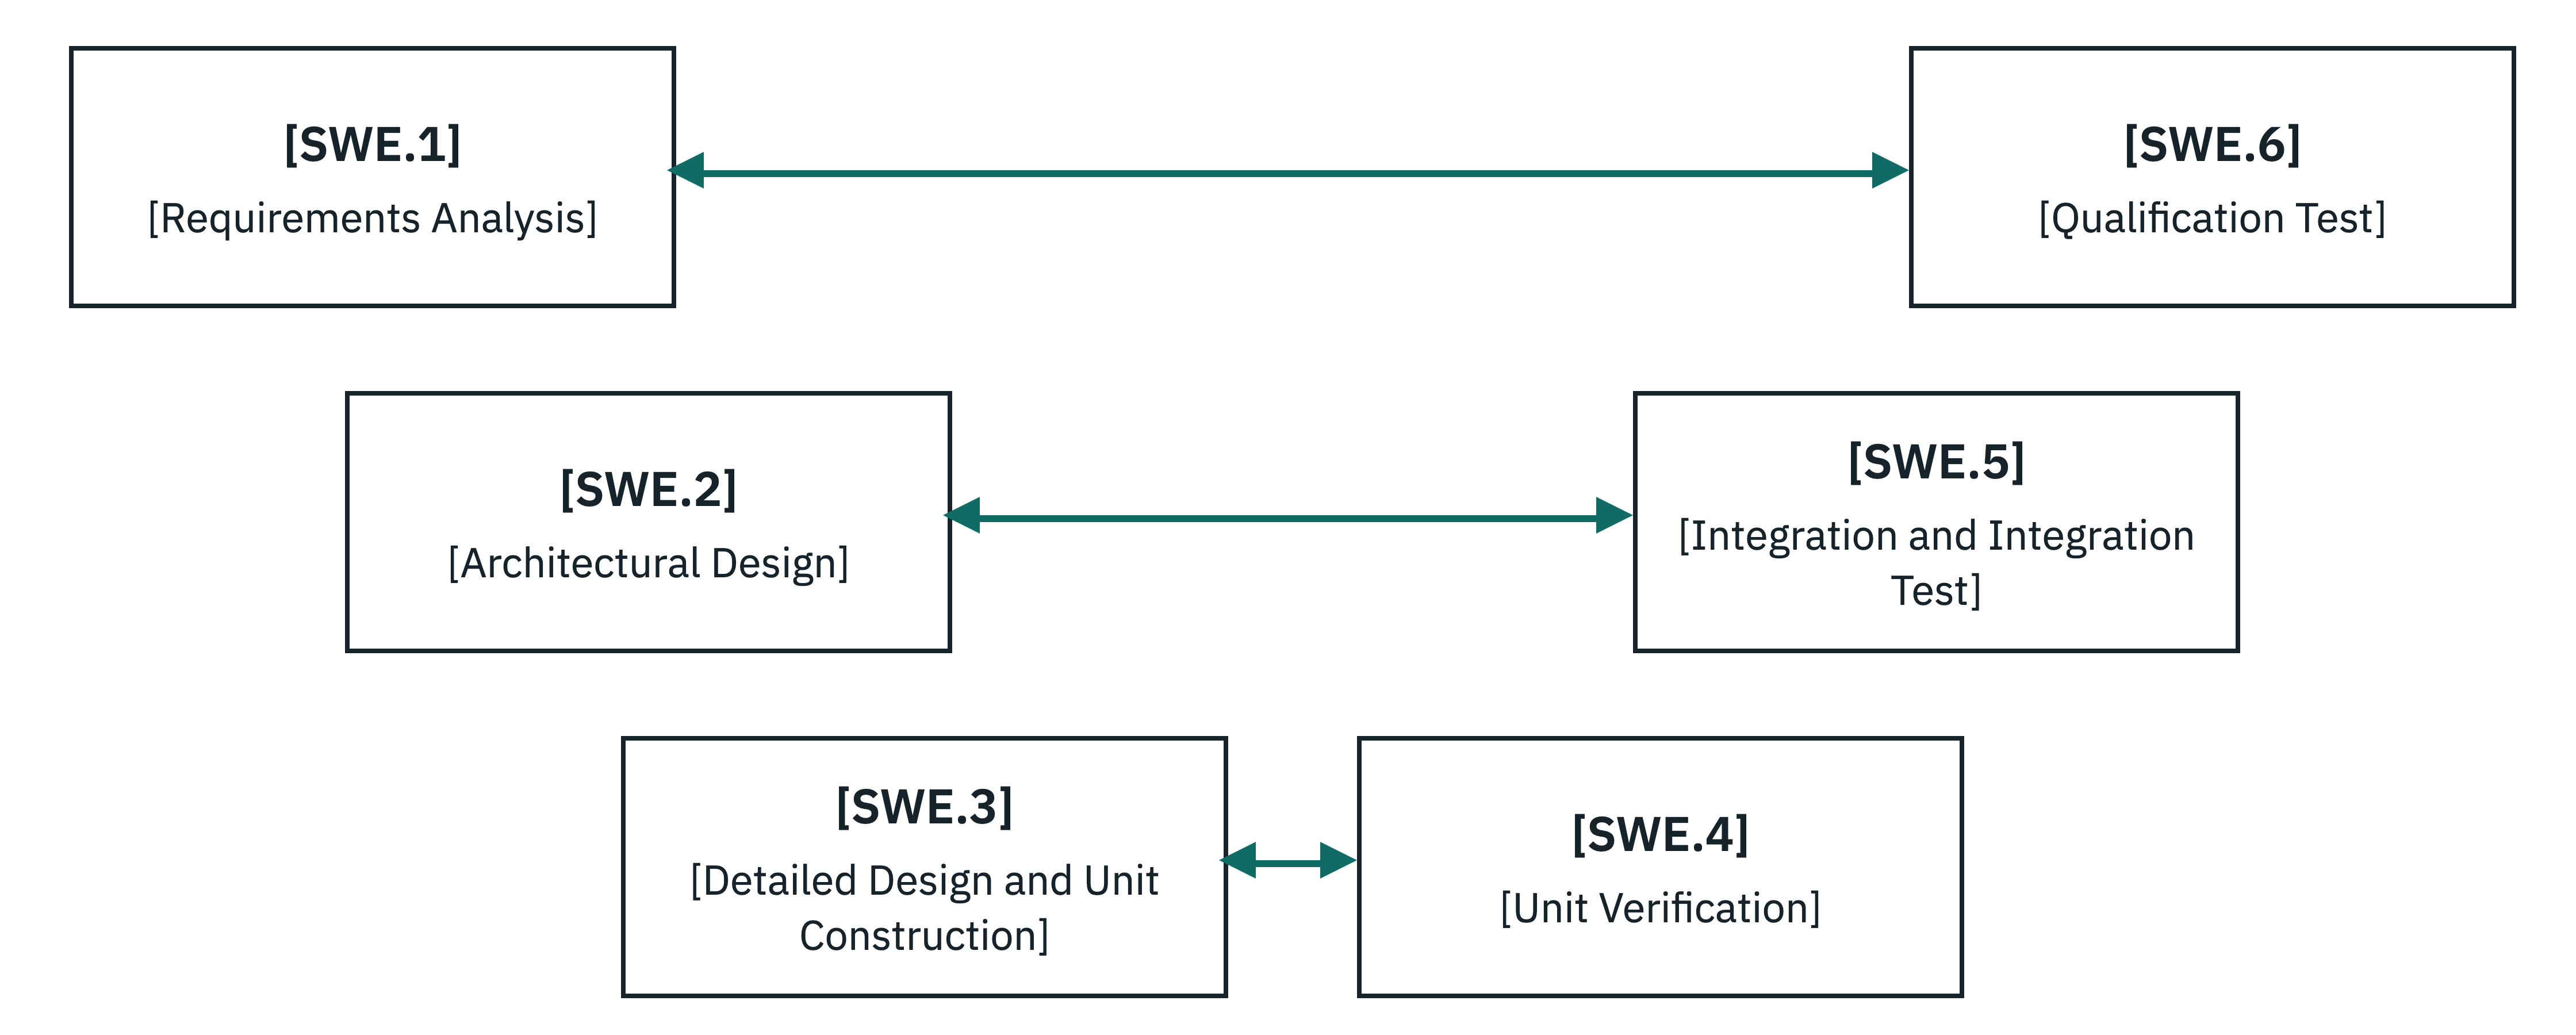
\includegraphics[width=0.6\textwidth]{src/v-model.png}
  \caption{The V-model view of the SWE.1--SWE.6 processes. Adapted from~\cite{vmodel_visure}.}
  \label{fig:v-model}
\end{figure}

\begin{description}
  \item[SWE.1 --- Software Requirements Analysis] Captures the software requirements from the
  system requirements and the system architecture.
  \item[SWE.2 --- Software Architectural Design] Defines the software architecture: how the
  software is split into components and how those components interact.
  \item[SWE.3 --- Software Detailed Design and Unit Construction] Designs each software unit in
  detail and implements it.
  \item[SWE.4 --- Software Unit Verification] Checks that each implemented unit matches its
  detailed design.
  \item[SWE.5 --- Software Integration and Integration Test] Integrates the verified units into
  larger components and the full software build, and tests that this integration works.
  \item[SWE.6 --- Software Qualification Test] Tests the fully integrated software against the
  original software requirements.
\end{description}

As Figure~\ref{fig:v-model} shows, the six processes pair up around this V-shape: SWE.1
(requirements) pairs with SWE.6 (software qualification test), SWE.2 (architecture) pairs with
SWE.5 (integration test), and SWE.3 (detailed design) pairs with SWE.4 (unit
verification)~\cite{vdaqmc2023pam}. Each process has its own base practices, the concrete
activities an assessor checks for, which this thesis uses directly as the source material for
its question bank (Chapter~\ref{chap:implementation}).

\subsection{Capability Levels and Base Practices (L1--L3)}

A process is not simply rated as present or absent. ASPICE defines six capability levels, shown
in Figure~\ref{fig:capability-levels}, and a process only reaches a given level once it also
satisfies every level below it~\cite{vdaqmc2023pam,vdaqmc_website}.

\begin{figure}[h]
  \centering
  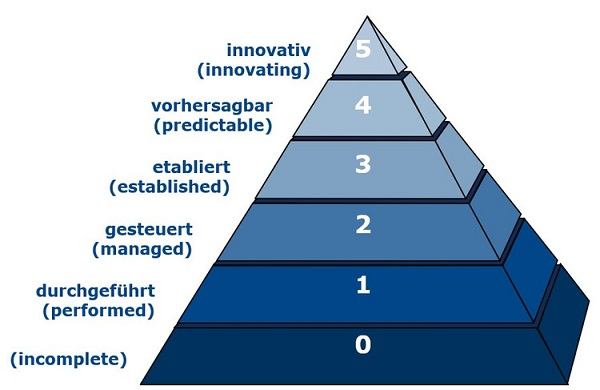
\includegraphics[width=0.45\textwidth]{src/levels.jpg}
  \caption{The six ASPICE capability levels, from Level~0 (Incomplete) to Level~5 (Innovating).
  Adapted from the official Automotive SPICE process model~\cite{vdaqmc_website}.}
  \label{fig:capability-levels}
\end{figure}

\begin{description}
  \item[L0, Incomplete] The process is not implemented, or fails to achieve its purpose.
  \item[L1, Performed] The process achieves its purpose. Evidence for this level comes from base
  practices, the process-specific activities defined for each of the SWE.1--SWE.6 processes.
  \item[L2, Managed] The process is not just performed but planned, monitored, and its work
  products are properly controlled.
  \item[L3, Established] The process follows a documented standard process, tailored and deployed
  consistently across the organization.
  \item[L4, Predictable] The process runs within defined quantitative limits, so its performance
  can be predicted.
  \item[L5, Innovating] The process is continuously improved, organization-wide, based on
  quantitative feedback.
\end{description}

This thesis covers the first three levels, L1--L3. Levels~L4 and~L5 are out of scope, since they
require evidence collected across many projects over time rather than evidence a single
stakeholder can report in one session~\cite{vdaqmc2023pam}.

\subsection{The Traditional (Manual) Assessment Procedure}

An ASPICE assessment is carried out by a certified assessor, who examines work products
(documents, models, test records) and interviews project staff to judge whether each base
practice and generic practice is satisfied. Each process attribute is then rated on a four-point
ordinal scale, from \emph{Not achieved} to \emph{Fully achieved}, based on the proportion of
evidence found~\cite{vdaqmc2023pam}. The result is a capability profile: a rating for every
process and level the assessment covered.

This procedure happens as a scheduled event, typically once or twice per project, and produces a
single point-in-time judgment~\cite{vdaqmc2023pam,murphy_aspice_0to60}. Between assessments, an
organization has no built-in mechanism, defined by the standard itself, for checking whether the
processes it was rated on are still being followed.

% TODO(figure): ASPICE PAM v4.0 Fig. 5 (p.28) -- "Performing a process assessment for
% determining process capability" (Execution -> Methods -> PAM, 3-step diagram). Redraw
% cleanly rather than screenshotting the PDF. Source: vdaqmc2023pam.

\subsection{Pain Points of Manual Assessment (Time, Consistency, Continuity)}

Three consequences follow from that procedure. First, feedback only exists at audit time: a
process weakness introduced the week after an assessment can go unnoticed until the next one.
Second, fixing a problem discovered late costs more than fixing the same problem early, because by
the time it surfaces, other work may already depend on the flawed
requirement or design~\cite{schauffele2016automotive,jiang2013earlylifecycle}. Third, the
depth of a manual assessment is limited by assessor time: with only a fixed number of days on
site, an assessor samples evidence rather than reviewing every artifact, so the coverage of any
single audit depends on which questions the assessor happens to ask. Dimitrios describes this
same gap directly: after certification, there is no direct way to monitor
whether a supplier's processes stay compliant, and organizations fall back on generic project
management or defect-tracking tools that were not built for process
assessment~\cite{datsogiannis2024early}. This is the specific problem the rest of the thesis
responds to.

% TODO(figure): 2025 supervisor paper, Fig. 1 -- "Process of bug finding and fixing in relation
% to time" (swimlane, bugfixing feedback loop). Illustrates the defect-cost-over-time point in
% the sentence above. Source: datsogiannis2025recommender. (Also usable in Ch.1 Motivation --
% place it in whichever section ends up needing the visual more.)

\section{Recommender Systems}

A recommender system selects a small, relevant subset of items from a much larger pool, for a
specific user and situation, instead of presenting the whole pool at
once~\cite{lu2012recommendersystems}. This thesis applies the same underlying idea to selecting
which ASPICE question to ask next.

\subsection{Content-Based and Collaborative Filtering Approaches}

Content-based filtering and collaborative filtering are the two classical
approaches~\cite{lu2012recommendersystems}, but neither fits this thesis directly: both need a
stable history of past preferences, either a stakeholder's own or other users', and a new
deployment of this system starts with no history for either the questions or the stakeholders
answering them. Chapter~\ref{chap:sota} discusses this comparison in more detail.

\subsection{Sequential and Adaptive Recommendation}

A better fit is sequential, adaptive recommendation: the system selects one item, observes the
outcome, and uses that outcome to decide the next selection, repeating this for the length of a
session. This is the model this thesis builds on, and it is what motivates the CMAB-based
approach described in the next section~\cite{datsogiannis2024early}; Chapter~\ref{chap:sota}
covers the prior work behind this choice in full.

\section{Multi-Armed Bandits}

A multi-armed bandit describes a repeated decision problem: on each round, an agent picks one
option out of several (an ``arm''), receives a reward for that choice, and tries to maximize its
total reward over time~\cite{naeem2020gentleintro,sutton2018reinforcement}. The name comes from a
row of slot machines (``one-armed bandits''), each with an unknown, possibly different payout
rate.

\subsection{The Exploration--Exploitation Trade-off}

The central difficulty in a bandit problem is that the agent cannot know in advance which arm
pays best. It has to spend some rounds trying arms it knows little about
(\emph{exploring}) and some rounds picking the arm that has performed best so far
(\emph{exploiting}), and it only ever observes the reward of the arm it actually
picked~\cite{datsogiannis2024early,naeem2020gentleintro}. Getting this balance wrong in either
direction is costly: exploiting too early risks settling on an arm that only looked good by
chance, while exploring too long wastes rounds on arms that are already known to be weak.

Several algorithms address this trade-off in different ways:

\begin{description}
  \item[Epoch-Greedy] Alternates fixed periods of exploration and
  exploitation~\cite{langford2007epochgreedy}.
  \item[Softmax / $\epsilon$-greedy] Chooses the current best arm most of the time, but picks a
  random arm with some fixed or decaying probability~\cite{tokic2011valuedifference}.
  \item[Thompson Sampling] Keeps a probability distribution over how good each arm might be, and
  samples from it to decide which arm to try~\cite{agrawal2013thompson}.
  \item[Upper Confidence Bound (UCB)] Adds a bonus to each arm's estimated reward that grows with
  how uncertain that estimate still is, so an arm gets tried more often either because it looks
  rewarding or because it has not been tried enough to be sure~\cite{auer2002confidence}.
\end{description}

\subsection{From Stateless Bandits to Contextual Bandits}

The algorithms above assume every round of the problem looks the same: the same set of arms, the
same underlying reward for each one. That assumption does not hold here. Which question is most
informative depends on who is answering (their stakeholder role), and on what has already
happened in the session so far, such as which processes and capability levels have already been
covered~\cite{datsogiannis2024early}.

A \emph{contextual} multi-armed bandit (CMAB) removes that assumption. Before each round, the
agent observes a context, a vector of features describing the current situation, and its estimate
of each arm's reward is allowed to depend on that context~\cite{li2010contextual}. In this
thesis, the context vector describes the stakeholder's role and the state of the current
assessment session; the full definition is given in Chapter~\ref{chap:architecture}. Framing
question selection this way lets the same pool of questions serve every stakeholder role,
because the algorithm learns which questions matter for which context rather than treating all
users identically~\cite{gutowski2018contextenhancement}.

% (The standard online-bandit-serving-loop diagram for this concept, Explore -> Join Service ->
% Learn Online -> Deploy, is now shown in Chapter 3, Figure~\ref{fig:soa-cmab-workflow}.)

\subsection{LinUCB --- Mathematical Foundations}

This thesis uses LinUCB, a contextual bandit algorithm that assumes each arm's expected reward is
a linear function of the context vector~\cite{li2010contextual,huang2016linucb}. For a context
vector $x$, arm $a$ maintains two learned quantities: a $d \times d$ matrix $A_a$ and a
$d$-dimensional vector $b_a$, where $d$ is the number of context features. From these, the
algorithm estimates a weight vector

\[
\theta_a = A_a^{-1} b_a ,
\]

and scores arm $a$ for the current context as

\[
\mathrm{UCB}_a(x) = \theta_a^\top x \; + \; \alpha \sqrt{x^\top A_a^{-1} x} .
\]

The first term, $\theta_a^\top x$, is the algorithm's current best estimate of the reward arm $a$
would give in this context. The second term grows when $A_a$ reflects little data for contexts
like $x$, so it rewards arms the algorithm is still uncertain about. The exploration coefficient
$\alpha$ controls how much weight that uncertainty bonus gets relative to the plain reward
estimate~\cite{li2010contextual}. At each round, LinUCB picks the arm with the highest
$\mathrm{UCB}_a(x)$.

After the chosen arm returns a reward $r$, its parameters are updated:

\[
A_a \leftarrow A_a + x x^\top , \qquad b_a \leftarrow b_a + r\, x .
\]

A question that has never been asked starts from $A_a = I$ (the identity matrix) and $b_a =
\mathbf{0}$, so every new question begins with the same, maximally uncertain estimate, and the
uncertainty bonus in $\mathrm{UCB}_a(x)$ is what gives it a fair chance of being selected the
first few times it is eligible~\cite{li2010contextual}. Because the update rule only involves
matrix and vector arithmetic, and the arm choice is a deterministic function of $A_a$, $b_a$, and
$x$, the same context and the same history always produce the same choice, which is one of the
properties that makes LinUCB a reasonable fit for a thesis that needs reproducible results.

\section{Chapter Summary}

ASPICE gives this thesis its domain: six software engineering processes, rated against base
practices at three capability levels, normally assessed by a person during a scheduled audit.
Recommender systems, and specifically the sequential, adaptive kind, give the general shape of a
solution: select a few informative questions instead of asking everything. Contextual bandits,
and LinUCB in particular, give the specific mechanism this thesis implements: a way to pick the
next question based on who is answering and what the session has covered so far, and to keep
improving that choice as more sessions are completed. Chapter~\ref{chap:sota} positions this
thesis against the closest existing work; Chapter~\ref{chap:architecture} shows how these three
pieces fit together in the actual system.

\chapter{State of the Art (12--17 pages)}
\label{chap:sota}
% \input{src/state_of_the_art}

This chapter positions this thesis against the closest existing work. It starts with a short
look at ASPICE and how it is assessed in current practice, then walks through the two papers by
Dimitrios that this thesis builds on most directly, together with the diagrams that describe
their approach. It closes with a comparison table and a statement of the research gap this
thesis addresses.

\section{ASPICE and Current Assessment Practice}

Chapter~\ref{chap:background} described how an ASPICE assessment is normally carried out. In
practice, that procedure runs as a periodic audit: a certified assessor visits a project at
defined milestones, samples evidence against the SWE.1--SWE.6 base practices, and produces a
capability rating that stays valid until the next
audit~\cite{vdaqmc2023pam,murphy_aspice_0to60}. This is the baseline the rest of this chapter
compares against. Dimitrios states its main limitation directly: ASPICE certification does
not come with a built-in way to monitor process compliance afterwards, so organizations fall
back on project management tools or defect-tracking systems that were never designed to check
whether a specific base practice is still being followed~\cite{datsogiannis2024early}. The next
section looks at how Dimitrios proposes to close that gap.

Figure~\ref{fig:soa-aspice-indicators} shows how the indicators behind that rating are actually
structured. A process's purpose and outcomes come from the PRM; the PAM then adds the evidence
an assessor collects to rate it. At Capability Level~1, that evidence is the process performance
indicators, base practices and work products, specific to each process. Above Level~1, it is the
process capability indicators, generic practices and generic resources, that apply the same way
across every process~\cite{vectorconsulting_aspice}.

\begin{figure}[h]
  \centering
  
\includegraphics[width=0.7\textwidth]{src/Soa_Aspice_1.png}
  \caption{How PRM and PAM indicators relate to capability levels: base practices and work
  products evidence Capability Level~1, while generic practices and generic resources evidence
  every level above it. Adapted from Vector Consulting~\cite{vectorconsulting_aspice}.}
  \label{fig:soa-aspice-indicators}
\end{figure}

\section{Prior Work: CMAB-Based Recommendation for Automotive Process Assessment}

Two papers by Dimitrios, from TU Chemnitz, propose using a contextual multi-armed bandit to
select assessment questions for automotive software processes.
The first introduces the concept and its architecture~\cite{datsogiannis2024early}; the second
extends it with a concrete comparison of bandit algorithms on simulated
data~\cite{datsogiannis2025recommender}. Both are the closest prior work to this thesis, and the
design in Chapter~\ref{chap:architecture} builds directly on them.

\subsection{2024 --- A Dynamic Survey Model for Automotive Process Evaluation}

Dimitrios proposes a recommendation system that manages a dynamic questionnaire instead of a
fixed one~\cite{datsogiannis2024early}. Questions are drawn from a
literature review covering automotive software development metrics, automotive-specific studies,
ASPICE (covering SYS.1--SYS.5, SWE.1--SWE.6, VAL.1, and PIM.3), ISTQB~\cite{istqb_website}, and
documented OEM electrical/electronic processes. Each question is assigned a weight reflecting its
importance, and each answer option a value; the value increases as the answer indicates a worse
outcome, so the highest-value answer is the one that most clearly reveals a weakness.
Figure~\ref{fig:soa-evaluation-packet} shows how a single question is packaged once it reaches
this stage: an identifier, the roles allowed to ask it and the roles affected by a failing
answer, its weight, the question and answer payloads, and the answer actually given.

\begin{figure}[h]
  \centering
  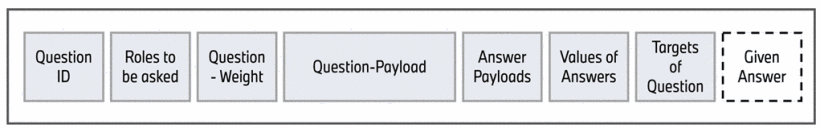
\includegraphics[width=\textwidth]{src/Soa_2.png}
  \caption{Structure of an evaluation packet, from question identifier to given answer.
  Reproduced from~\cite{datsogiannis2024early}.}
  \label{fig:soa-evaluation-packet}
\end{figure}

A CMAB agent then selects which questions to ask, and to which of seven stakeholder roles, during
each development cycle. Figure~\ref{fig:soa-cmab-workflow} shows this as a continuous serving
loop rather than a one-off computation: the agent explores using the current context, the
resulting context, action, and reward are logged and joined into training data, a new model is
learned online from that data, and the updated model is deployed back into the agent before the
next round.

\begin{figure}[h]
  \centering
  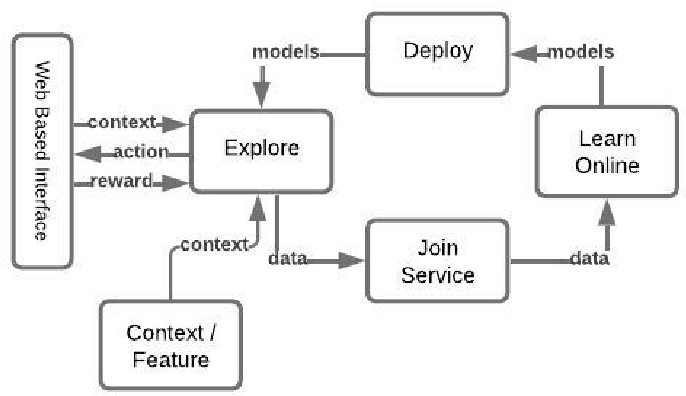
\includegraphics[width=0.65\textwidth]{src/Soa_3.png}
  \caption{The CMAB serving loop: explore, log context/action/reward, learn a new model online,
  deploy it, and explore again. Reproduced from~\cite{datsogiannis2024early}.}
  \label{fig:soa-cmab-workflow}
\end{figure}

The paper also proposes a three-band traffic-light classification of results (red, yellow,
green), based on two thresholds applied to a computed score. It stops short of a full
implementation: its own conclusion states that the concept was still being developed at the time
of publication, and that training and evaluation results would be reported later~\cite{datsogiannis2024early}.

\textbf{Relevance to this thesis.} Two design choices from this paper carry over directly. First,
every question carries a weight and every answer a value, so that a session's raw answers can be
turned into a numeric score without further interpretation. Second, the reward given to the CMAB
agent is built so that the worst answer to the most important question produces the highest
reward, deliberately pointing the agent toward questions likely to expose a real weakness rather
than questions that are merely easy to answer. Chapter~\ref{chap:architecture} refines the
three-band classifier into a four-band scheme, and, unlike this paper, actually implements and
runs the resulting system.

\subsection{2025 --- Algorithm Benchmarking on Simulated Data}

Dimitrios extends the same concept with a question pool of 137 questions and a direct
comparison of three bandit algorithms: $\epsilon$-greedy, LinUCB, and Thompson
Sampling~\cite{datsogiannis2025recommender}. Since no real deployment existed yet, the comparison
runs in a simulated environment built to resemble the behavior of real software releases. Four
scenarios vary how much the underlying set of process deficiencies changes between evaluation
rounds: a stable scenario (0\% change), and three scenarios in which 10\%, 30\%, or 50\% of the
deficiencies change from one round to the next. Each algorithm was tuned separately for each
scenario, as summarized in Figure~\ref{fig:soa-tuning-tree}, then compared over 1{,}000 simulated
rounds using three measures: cumulative reward, average reward per round, and the share of
rewards falling into four score bands, illustrated for one scenario in
Figure~\ref{fig:soa-reward-distribution}. Table~\ref{tab:recommender-results} reproduces the
result for the least and most volatile scenarios, using each algorithm's own best tuning.

\begin{figure}[h]
  \centering
  
\includegraphics[width=0.9\textwidth]{src/Soa_4.png}
  \caption{Best tuning parameter found for each of the three algorithms, in each of the four
  deficiency-change scenarios. Reproduced from~\cite{datsogiannis2025recommender}.}
  \label{fig:soa-tuning-tree}
\end{figure}

\begin{figure}[h]
  \centering
  
\includegraphics[width=0.5\textwidth]{src/Soa_5.png}
  \caption{Distribution of $\epsilon$-greedy's rewards at 0\% deficiency change, across four
  score bands. Reproduced from~\cite{datsogiannis2025recommender}.}
  \label{fig:soa-reward-distribution}
\end{figure}

\begin{table}[h]
\centering
\caption{Simulated algorithm comparison at 0\% and 50\% deficiency-change rate, reproduced
from~\cite{datsogiannis2025recommender}. The right-hand column is the share of rewards that fell
above 0.75, the band representing the most important questions paired with the worst answers.}
\label{tab:recommender-results}
\begin{tabular}{|l|l|c|c|}
\hline
\textbf{Scenario} & \textbf{Algorithm} & \textbf{Tuning} & \textbf{Rewards $>$ 0.75} \\
\hline
0\% change  & $\epsilon$-greedy & $\epsilon=0.5$ & 47.2\% \\
            & LinUCB            & $\alpha=0.1$   & 34.4\% \\
            & Thompson Sampling & $\alpha=0.5$   & 36.7\% \\
\hline
50\% change & $\epsilon$-greedy & $\epsilon=0.5$ & 25.3\% \\
            & LinUCB            & $\alpha=0.1$   & 24.3\% \\
            & Thompson Sampling & $\alpha=5.0$   & 23.9\% \\
\hline
\end{tabular}
\end{table}

The pattern in Table~\ref{tab:recommender-results} holds across all four scenarios:
$\epsilon$-greedy has the highest share of high-reward outcomes throughout, though its advantage
over LinUCB narrows as the deficiency-change rate rises, from about 13 percentage points at 0\%
change to about 1 percentage point at 50\% change~\cite{datsogiannis2025recommender}. LinUCB's own
best tuning parameter, $\alpha$, also varies by scenario, from $\alpha=0.1$ in most scenarios up
to $\alpha=2.0$ in the 30\%-change scenario. Neither result comes from a real deployment: the
paper's own conclusion states that a further publication would report results from a real
automotive development environment~\cite{datsogiannis2025recommender}.

\textbf{Relevance to this thesis.} This is the closest existing evidence on how LinUCB, the
algorithm this thesis uses, actually performs against alternatives, and it is a benchmark this
thesis cannot ignore simply because LinUCB did not win it. Section~\ref{sec:cross-comparison}
weighs that result against this thesis's own reasons for choosing LinUCB regardless.

\section{Cross-Comparison and the Recommended Method for This Thesis}
\label{sec:cross-comparison}

Table~\ref{tab:cross-comparison} compares manual ASPICE practice, the prior work described above,
and this thesis, across the properties that matter for continuous, automated process assessment.
A \cmark\ marks a property the column satisfies and a \xmark\ marks one it does not; the
remaining rows describe properties that are not simply binary. Manual practice and the prior work
each satisfy some criteria but not all; this thesis is the only one of the three that satisfies
every checkable criterion at once, precisely because it narrows scope in exchange for actually
being implemented and evaluated.

\begin{table}[h]
\centering
\caption{Manual ASPICE practice, prior CMAB-based work, and this thesis, compared.}
\label{tab:cross-comparison}
\rowcolors{2}{green!5}{white}
\begin{tabular}{|p{2.7cm}|p{3.0cm}|p{3.6cm}|p{3.6cm}|}
\hline
\rowcolor{green!55!black}
\textcolor{white}{\textbf{Aspect}} & \textcolor{white}{\textbf{ASPICE (current practice)}} &
\textcolor{white}{\textbf{Prior work~\cite{datsogiannis2024early,datsogiannis2025recommender}}} &
\textcolor{white}{\textbf{This thesis}} \\
\hline
Assessment style & Manual, audit-driven & Continuous, question-driven & Continuous,
ASPICE-aligned, web-based \\
\hline
Question-based evaluation & \cmark\ Yes, by auditors & \cmark\ Yes, derived from metrics &
\cmark\ Yes, ASPICE base practices turned into questions \\
\hline
Structured question database & \xmark\ Not a standardized dataset & \cmark\ Generic questions for
general software & \cmark\ New structured SWE.1--SWE.6 question bank \\
\hline
ASPICE scope / focus & \cmark\ Full standard, as needed & \xmark\ SYS.1--SYS.5, SWE.1--SWE.6,
VAL.1, PIM.3 (not SWE-specific) & \cmark\ Explicit SWE.1--SWE.6 mapping only \\
\hline
Automated question selection & \xmark\ Human assessor selects & \cmark\ CMAB agent (three
algorithms compared) & \cmark\ CMAB agent (LinUCB) \\
\hline
Early feedback & \xmark\ Mostly late, at audit time & \cmark\ Early evaluation, in simulation &
\cmark\ Early SWE weakness visibility \\
\hline
Evaluation basis & Not applicable (the standard itself) & \xmark\ Simulated data only & \cmark\
Real pilot audit sessions \\
\hline
\end{tabular}
\end{table}

This thesis makes three deliberate choices relative to that prior work. First, it narrows the
ASPICE scope from four process groups to one, SWE.1--SWE.6, so that the question bank in
Chapter~\ref{chap:implementation} can be built directly from that group's base practices rather
than from a broader literature review. Second, it adopts LinUCB specifically, rather than
comparing multiple algorithms, because a deterministic selection rule is easier to reproduce and
reason about within a single thesis's evaluation, even though Table~\ref{tab:recommender-results}
shows $\epsilon$-greedy performing better in simulation; this trade-off is revisited in
Chapter~\ref{chap:results}. Third, it evaluates the system on real, non-simulated pilot sessions,
which neither prior paper does.

Recommender systems for automotive processes are not otherwise well covered in the literature.
The closest non-supervisor prior work is Bader's dissertation on proactive recommender systems in
automotive scenarios~\cite{bader2013proactive}, which addresses in-vehicle recommendation to
drivers rather than process assessment for development teams, and is not built on ASPICE.

\section{Research Gap}

Putting the previous sections together: manual ASPICE assessment has no continuous monitoring
mechanism~\cite{datsogiannis2024early}. The closest prior work proposes a continuous, CMAB-driven
alternative, but has not been implemented as a working system and has only been evaluated in
simulation~\cite{datsogiannis2024early,datsogiannis2025recommender}. No published work combines a
continuous, automated, stakeholder-driven recommendation system with an explicit implementation
of ASPICE SWE.1--SWE.6 and an evaluation on real assessment sessions. That is the gap this thesis
fills.

\section{Chapter Summary}

Manual ASPICE assessment gives clear ratings, but only at audit time. The prior work reviewed in
this chapter shows that a CMAB-driven questionnaire is workable in concept and in simulation, but
stops short of a real implementation. This thesis fills that space for SWE.1--SWE.6 specifically:
the same underlying idea, narrowed in ASPICE scope, committed to one algorithm, and tested on real
sessions rather than simulated ones. Chapter~\ref{chap:architecture} describes how that system is
built.

\chapter{System Architecture and Design (10--12 pages)}
\label{chap:architecture}
% \input{src/architecture}

This chapter describes how the system is designed, before Chapter~\ref{chap:implementation}
covers how it is actually built. It starts with the requirements the system has to satisfy, then
works through the overall architecture, the question bank and assessment model, the database
design, the CMAB recommendation engine, and the weakness classifier that turns stakeholder
answers into a result. It also covers the API and user interface design, and closes with the key
design decisions and trade-offs behind the system.

\section{Requirements Analysis}
\label{sec:requirements-analysis}

\subsection{Functional Requirements}

\begin{itemize}
  \item \textbf{FR1.} The system shall replace the manual, periodic ASPICE assessment
  procedure with a continuous, automated one, while remaining aligned with the ASPICE
  SWE.1--SWE.6 standard.
  \item \textbf{FR2.} Stakeholders shall be able to sign up, log in, and participate in an
  assessment session.
  \item \textbf{FR3.} The system shall maintain a structured question bank covering ASPICE
  SWE.1--SWE.6.
  \item \textbf{FR4.} The system shall ask each stakeholder only the questions relevant to
  their specific role.
  \item \textbf{FR5.} The system shall compute, automatically, where process weaknesses exist.
  \item \textbf{FR6.} The system shall present the assessment results clearly to the
  stakeholder.
\end{itemize}

\subsection{Non-Functional Requirements}

\begin{itemize}
  \item \textbf{NFR1 (Determinism).} Question selection shall be deterministic, given the same
  context and model state, so that results are reproducible.
  \item \textbf{NFR2 (Traceability).} Every question shall be traceable to a specific ASPICE
  SWE.1--SWE.6 base practice.
  \item \textbf{NFR3 (Security).} Access to the system shall require authentication.
  \item \textbf{NFR4 (Bounded session length).} An assessment session shall stay within a fixed
  question budget, so it takes a stakeholder only a short, predictable amount of time.
\end{itemize}

Table~\ref{tab:fr-traceability} maps each functional requirement back to the research question
it serves, so that the design decisions in the rest of this chapter can be read as direct answers
to Chapter~\ref{chap:introduction}'s research questions rather than as free-standing choices.

\begin{table}[h]
\centering
\caption{Functional requirements mapped to the research questions from
Chapter~\ref{chap:introduction}.}
\label{tab:fr-traceability}
\begin{tabular}{|c|p{9.5cm}|c|}
\hline
\textbf{Req.} & \textbf{Requirement} & \textbf{RQ} \\
\hline
FR1 & Continuous, automated, ASPICE-aligned assessment (core objective) & RQ1--RQ4 \\
\hline
FR2 & Stakeholder signup, login, and session participation (supporting infrastructure) & --- \\
\hline
FR3 & Structured SWE.1--SWE.6 question bank & RQ1 \\
\hline
FR4 & Role-targeted question selection & RQ2 \\
\hline
FR5 & Automatic weakness computation & RQ3 \\
\hline
FR6 & Clear presentation of results & RQ4 \\
\hline
\end{tabular}
\end{table}

% Optional (not yet added): a UML use-case diagram (actors: Stakeholder, Administrator; use
% cases: Start Session, Answer Question, View Results, View History, Manage Question Bank,
% View Analytics) would visualize this requirements section, but would be a fifth diagram in an
% already diagram-dense, 10--12 page chapter -- add only if there is room after writing the
% rest of the chapter.

\section{System Architecture}

\subsection{Overall Architecture}

Figure~\ref{fig:overall-architecture} shows the system at its highest level of abstraction. The
diagram is the same concept architecture originally proposed for this line of
work~\cite{datsogiannis2024early}, and it still describes this thesis's own system accurately:
development stakeholders and their manager interact with the system through a \emph{GUI}, every
request passes through a central \emph{Model Controller}, question selection is delegated to a
\emph{Recommendation System}, an \emph{Evaluation Model} turns answers into a result, and all
persistent state lives in a \emph{Database}.

\begin{figure}[h]
  \centering
  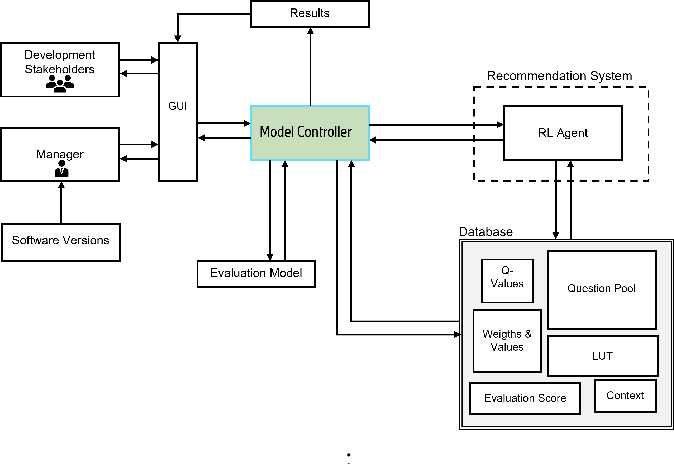
\includegraphics[width=0.85\textwidth]{src/Arch_1.png}
  \caption{Overall system architecture: stakeholders interact through the GUI, the Model
  Controller coordinates the Recommendation System (CMAB agent) and the Evaluation Model, and
  all state is persisted in the database. Adapted from the concept architecture
  proposed in~\cite{datsogiannis2024early}.}
  \label{fig:overall-architecture}
\end{figure}

Mapped onto the system actually built for this thesis, each box is a concrete component. The
\emph{GUI} is the React frontend. The \emph{Model Controller} is the FastAPI backend's business
logic, specifically the audit session service that coordinates a session from start to
completion. The \emph{Recommendation System} is the CMAB engine described in
Section~\ref{sec:cmab-engine}, using LinUCB to select questions. The \emph{Evaluation Model} is
the weakness classifier described in Section~\ref{sec:weakness-classification}. The \emph{Database}
is the PostgreSQL data layer, and its four labelled sub-parts correspond directly to this
thesis's own persisted state: \emph{Question Pool} and \emph{Weights \& Values} are the
\texttt{AuditQuestion}/\texttt{AuditOption} tables, \emph{Context} and \emph{Q-Values} are the
CMAB context vector and the learned \texttt{BanditArmState} parameters, and \emph{Evaluation
Score} is the computed \texttt{WeaknessResult}. One simplification is worth naming: the original
diagram treats ``Development Stakeholders'' and ``Manager'' as separate actor types and
``Software Versions'' as a distinct input; this thesis instead treats every stakeholder
uniformly through a single \texttt{stakeholder\_role} field on the user account, and each audit
session is a self-contained assessment cycle rather than one explicitly tied to a tracked
software release.

\subsection{System Components and Responsibilities}

Figure~\ref{fig:component-responsibilities} shows the same architecture from a responsibilities
point of view: what each component is actually accountable for, independent of the request flow
between them.

\begin{figure}[h]
  \centering
  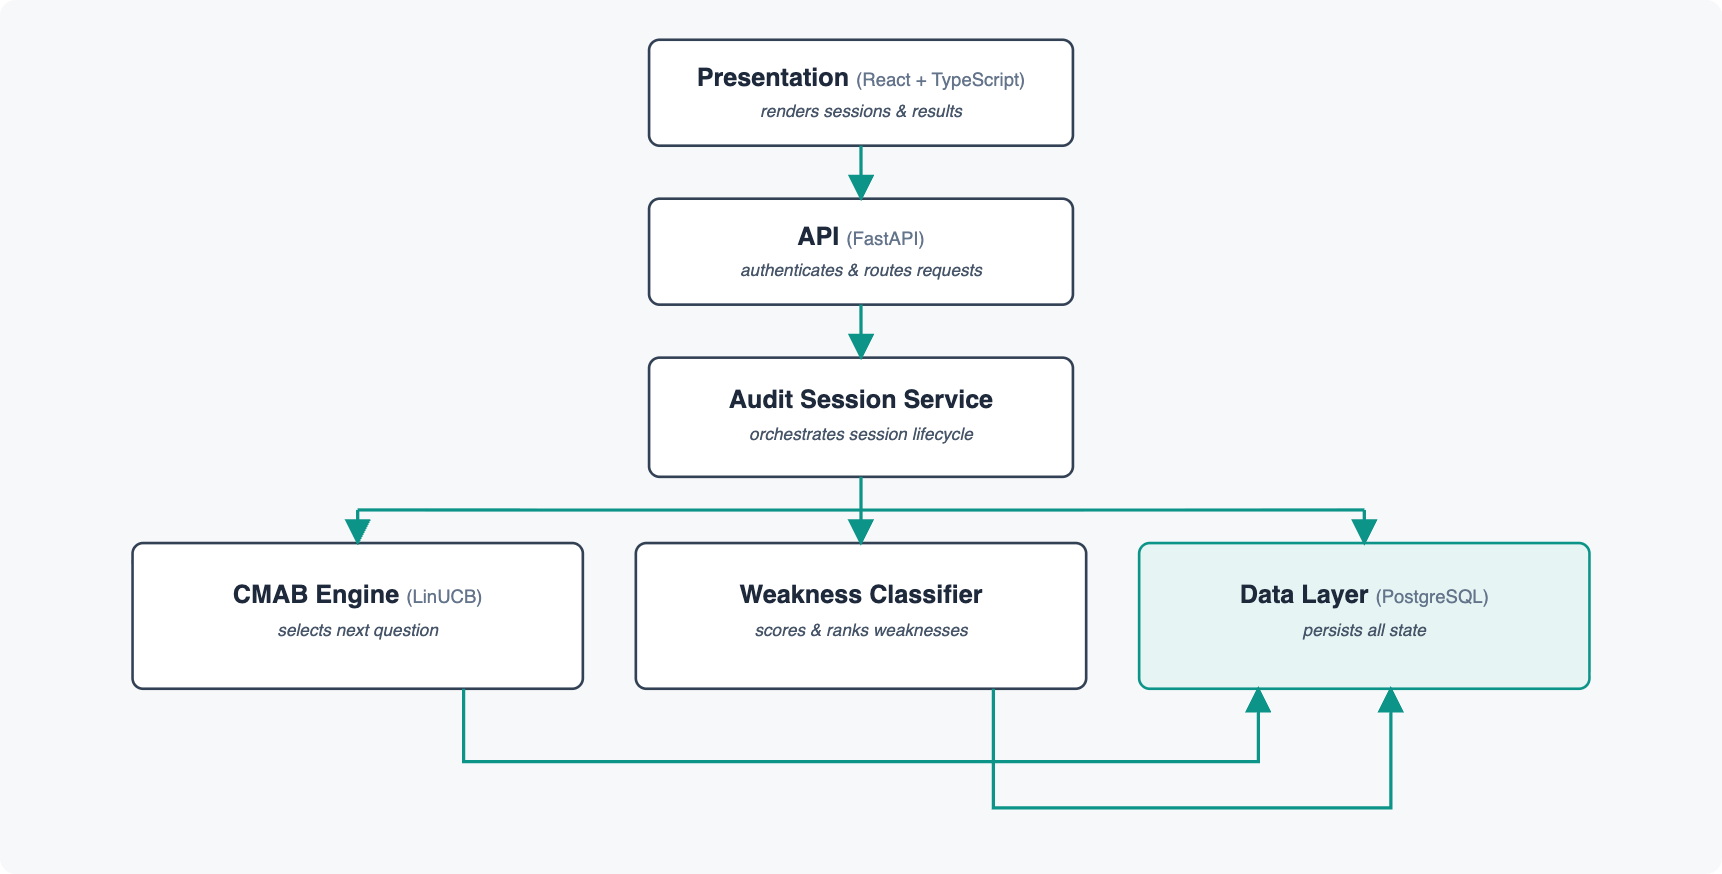
\includegraphics[width=0.85\textwidth]{src/Arch_2.png}
  \caption{System components and their responsibilities.}
  \label{fig:component-responsibilities}
\end{figure}

\subsection{Data and Control Flow}

Figure~\ref{fig:data-control-flow} traces a single answer-submission request through the system.
Solid arrows are control flow and dashed arrows are data reads and writes. A stakeholder's
answer moves from the presentation layer through the API to the audit session service, which
updates the CMAB engine and, depending on whether the session's question budget has been
reached, either receives the next question back from the CMAB engine or hands off to the
weakness classifier; every component along the way reads from or writes to the data layer.

\begin{figure}[h]
  \centering
  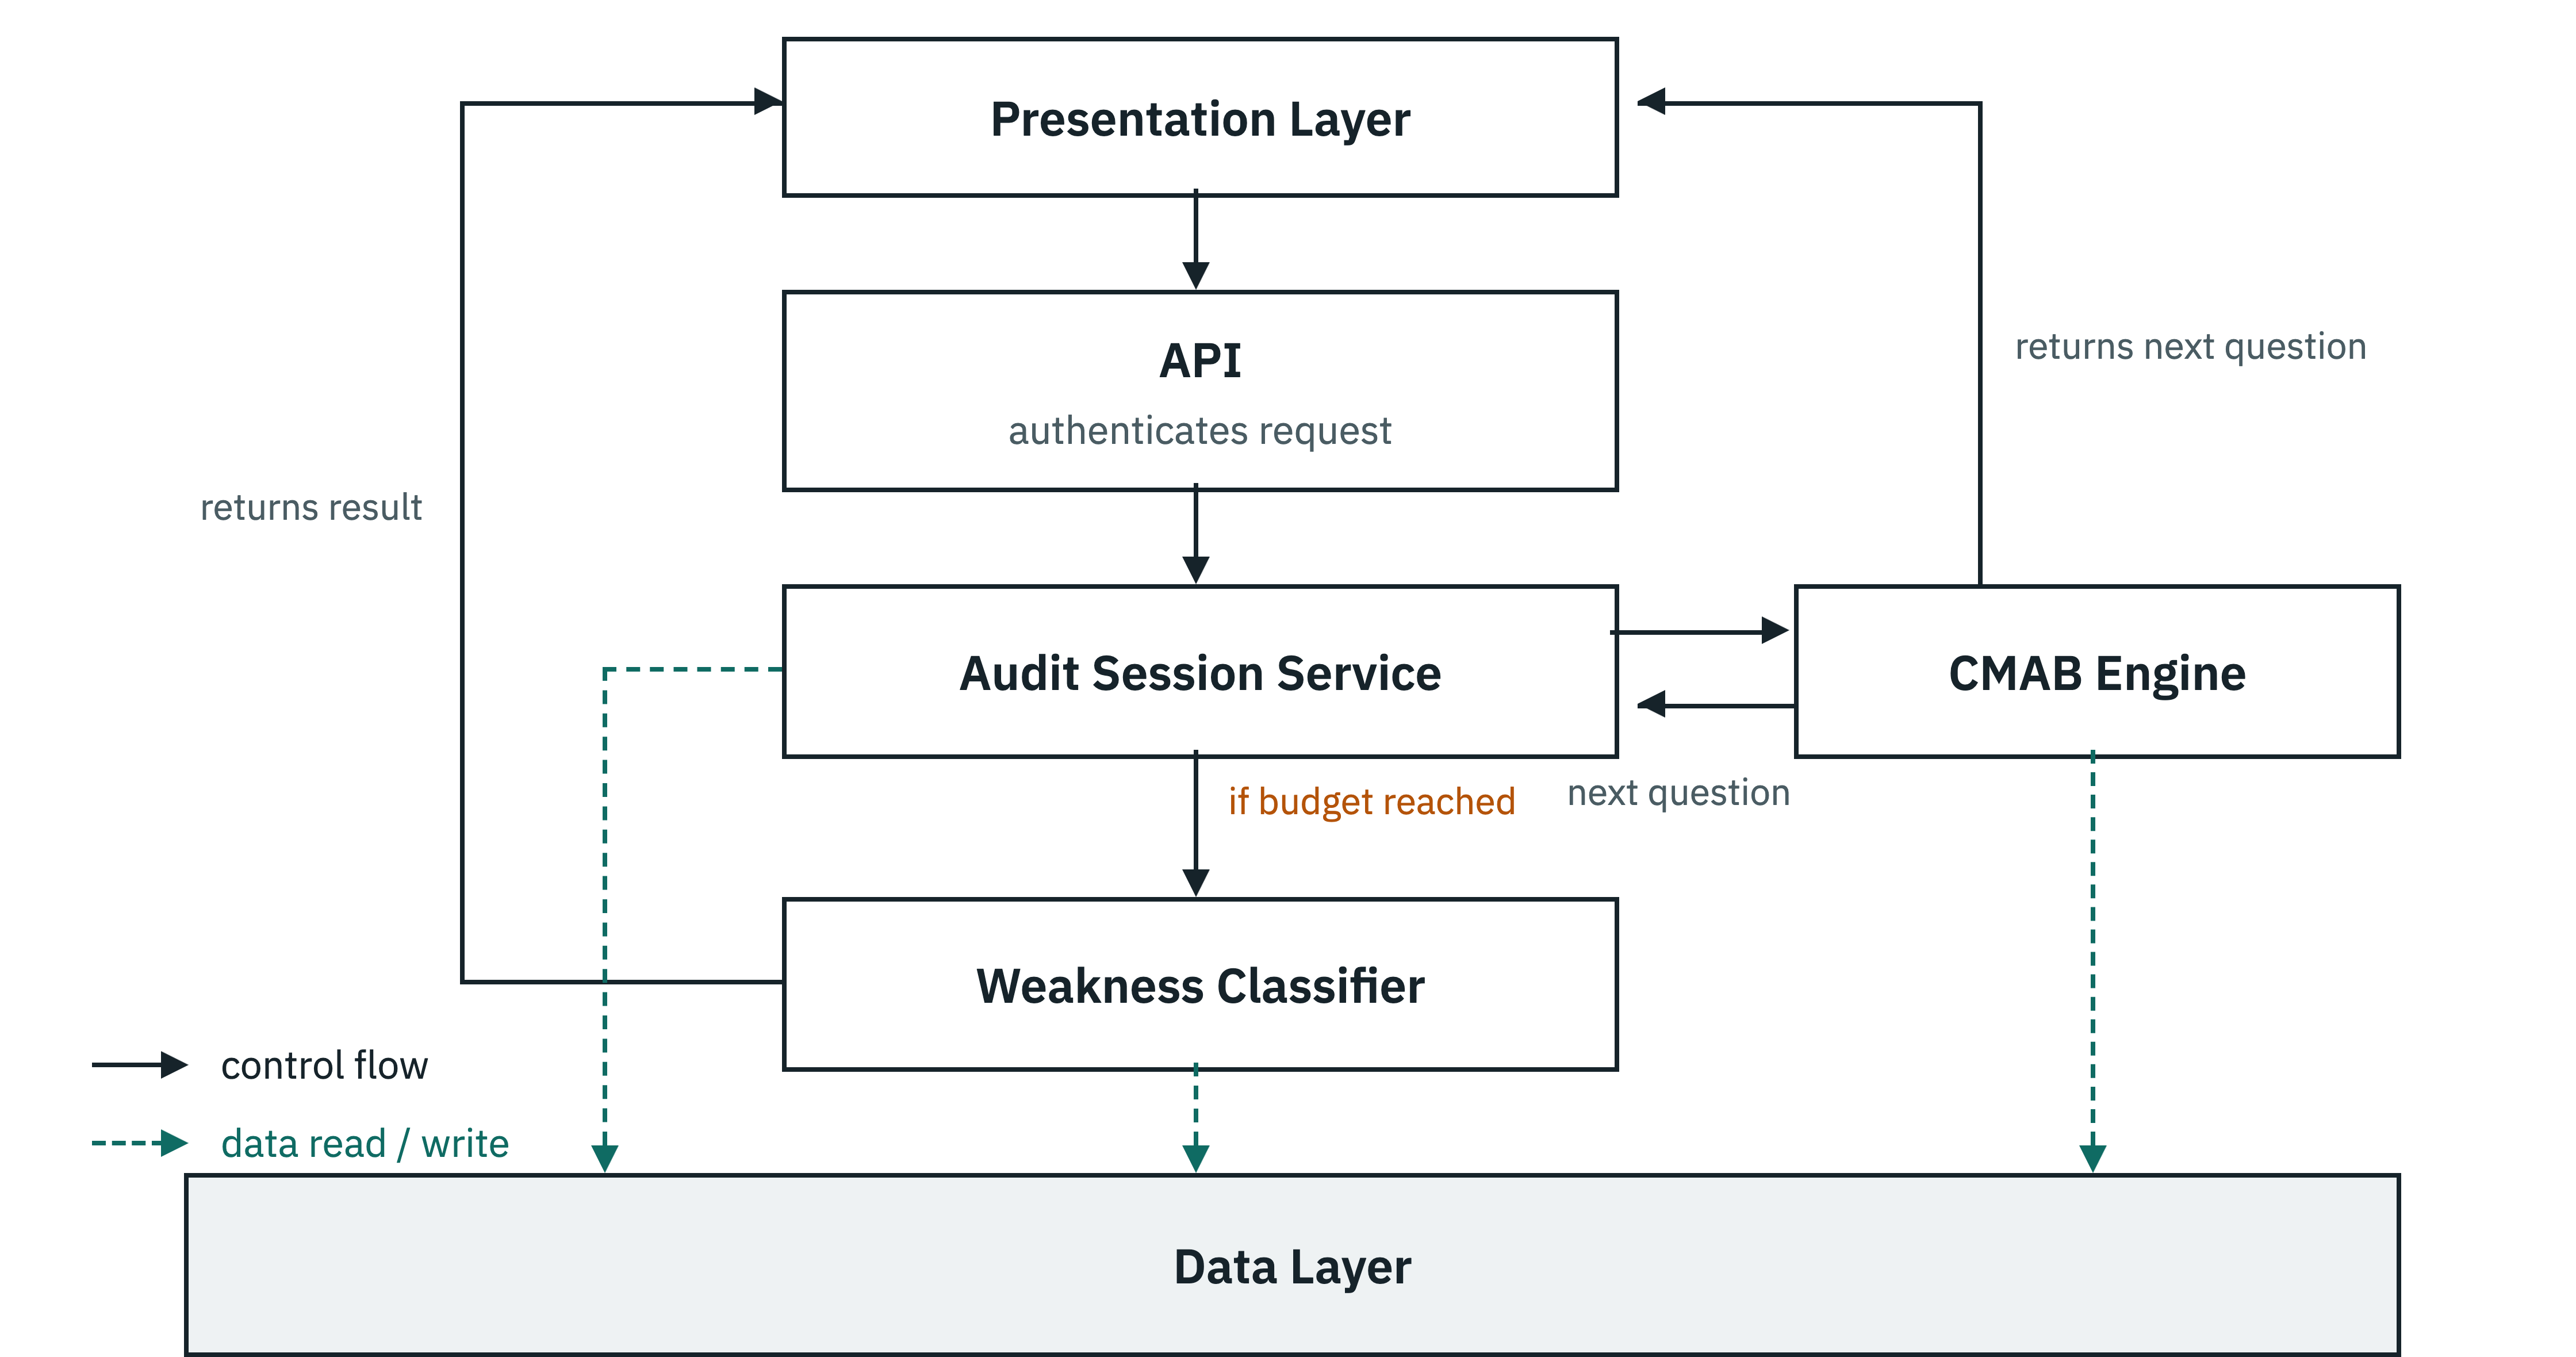
\includegraphics[width=0.75\textwidth]{src/Arch_3.png}
  \caption{Control and data flow for a single answer-submission request.}
  \label{fig:data-control-flow}
\end{figure}

Section~\ref{sec:api-design} and Section~\ref{sec:weakness-classification} revisit this same
flow at finer granularity, once the API contract and the classification logic have been
introduced.

\section{Question Bank and Assessment Model}

The question bank turns the ASPICE standard into something a stakeholder can actually answer.
This section explains how, using one seeded question, \texttt{SWE1\_L1\_01}, as a running
example.

\subsection{ASPICE Base Practice to Question Transformation}

Building the question bank means working through each SWE process's base practices, as defined
in the PAM~\cite{vdaqmc2023pam}, and rephrasing each one from an assessor's checklist item into a
question a stakeholder can answer about their own current work. SWE.1's first base practice
reads: ``\emph{Specify software requirements}\ldots\ per defined characteristics (verifiability,
unambiguity, freedom from design/implementation, no contradictions)''~\cite{vdaqmc2023pam}. This
becomes \texttt{SWE1\_L1\_01}: \emph{``How are software requirements specified for the current
release?''} The base practice's own characteristics are not repeated in the question text; they
reappear as the distinctions between its answer options.

\subsection{Question Structure and Traceability}

Every question is stored with a fixed structure: a unique code, its process and capability
level, the \texttt{base\_practice\_id} that ties it back to the PAM, the question text, and a
recommendation shown when an answer indicates a weakness. \texttt{SWE1\_L1\_01} traces to
\texttt{SWE.1.BP1}, and its recommendation is to introduce a requirement-specification template
and audit the tooling used to manage requirements. This traceability field is what satisfies
NFR2 from Section~\ref{sec:requirements-analysis}: any question's justification against the
standard is one lookup away.

\subsection{Answer Options and Weighting}
\label{sec:answer-weighting}

Each question has five predefined answer options, A through E, ordered from the strongest
practice to its complete absence, each carrying a weight from 0 (fully in place) up to 5
(effectively absent). Table~\ref{tab:example-question} shows the full set for
\texttt{SWE1\_L1\_01}. This weight is what the CMAB engine turns into a reward once an option is
selected, and what the weakness classifier later averages into a process score
(Sections~\ref{sec:cmab-engine} and~\ref{sec:weakness-classification}).

\begin{table}[h]
\centering
\caption{Answer options and weights for the worked example question \texttt{SWE1\_L1\_01}.}
\label{tab:example-question}
\begin{tabular}{|c|p{8.5cm}|c|}
\hline
\textbf{Option} & \textbf{Answer text} & \textbf{Weight} \\
\hline
A & Each requirement is uniquely identified, atomic, verifiable, and references its source & 0 \\
\hline
B & Requirements are uniquely identified but verifiability criteria are missing for some & 2 \\
\hline
C & Requirements exist as free-text paragraphs without unique IDs & 3 \\
\hline
D & Requirements are partially captured in slides or e-mails & 4 \\
\hline
E & No formal software requirements set exists & 5 \\
\hline
\end{tabular}
\end{table}

\subsection{Stakeholder Role Assignment}

Every question also carries one or more of seven stakeholder roles: Software Developer,
Software Architect, Project Manager, QA Engineer, Test Engineer, Team Lead, or ASPICE Assessor.
\texttt{SWE1\_L1\_01} is assigned to Software Architect, Software Developer, and QA Engineer, the
roles most likely to know how requirements are actually specified; a Project Manager is never
shown it. This is what lets one shared question bank serve every stakeholder without asking
anyone about work outside their own area, satisfying FR4 from
Section~\ref{sec:requirements-analysis}.

\subsection{Question-to-Assessment Flow}

Once structured, weighted, and role-tagged, a question is ready for use. At the start of a
session, and after every answer, the system filters to questions still eligible for the
stakeholder's role and not yet asked, and the CMAB engine (Section~\ref{sec:cmab-engine}) treats
each eligible question as one arm and selects among them. The same fields set at design time are
exactly what the eligibility filter and the weakness classifier read at runtime.

\section{Database Design}

Everything described so far, the question bank, the roles, the weights, has to live somewhere
between one request and the next, and has to be shared by every stakeholder who ever starts a
session. This section describes the seven tables that hold that state, and, more importantly,
why they are split the way they are.

\subsection{Entity-Relationship Model}

Figure~\ref{fig:erd} shows the full schema. The dashed boundary marks the two tables that hold
learned or derived state, \texttt{WeaknessResult} and \texttt{BanditArmState}, rather than
directly recorded stakeholder input.

\begin{figure}[h]
  \centering
  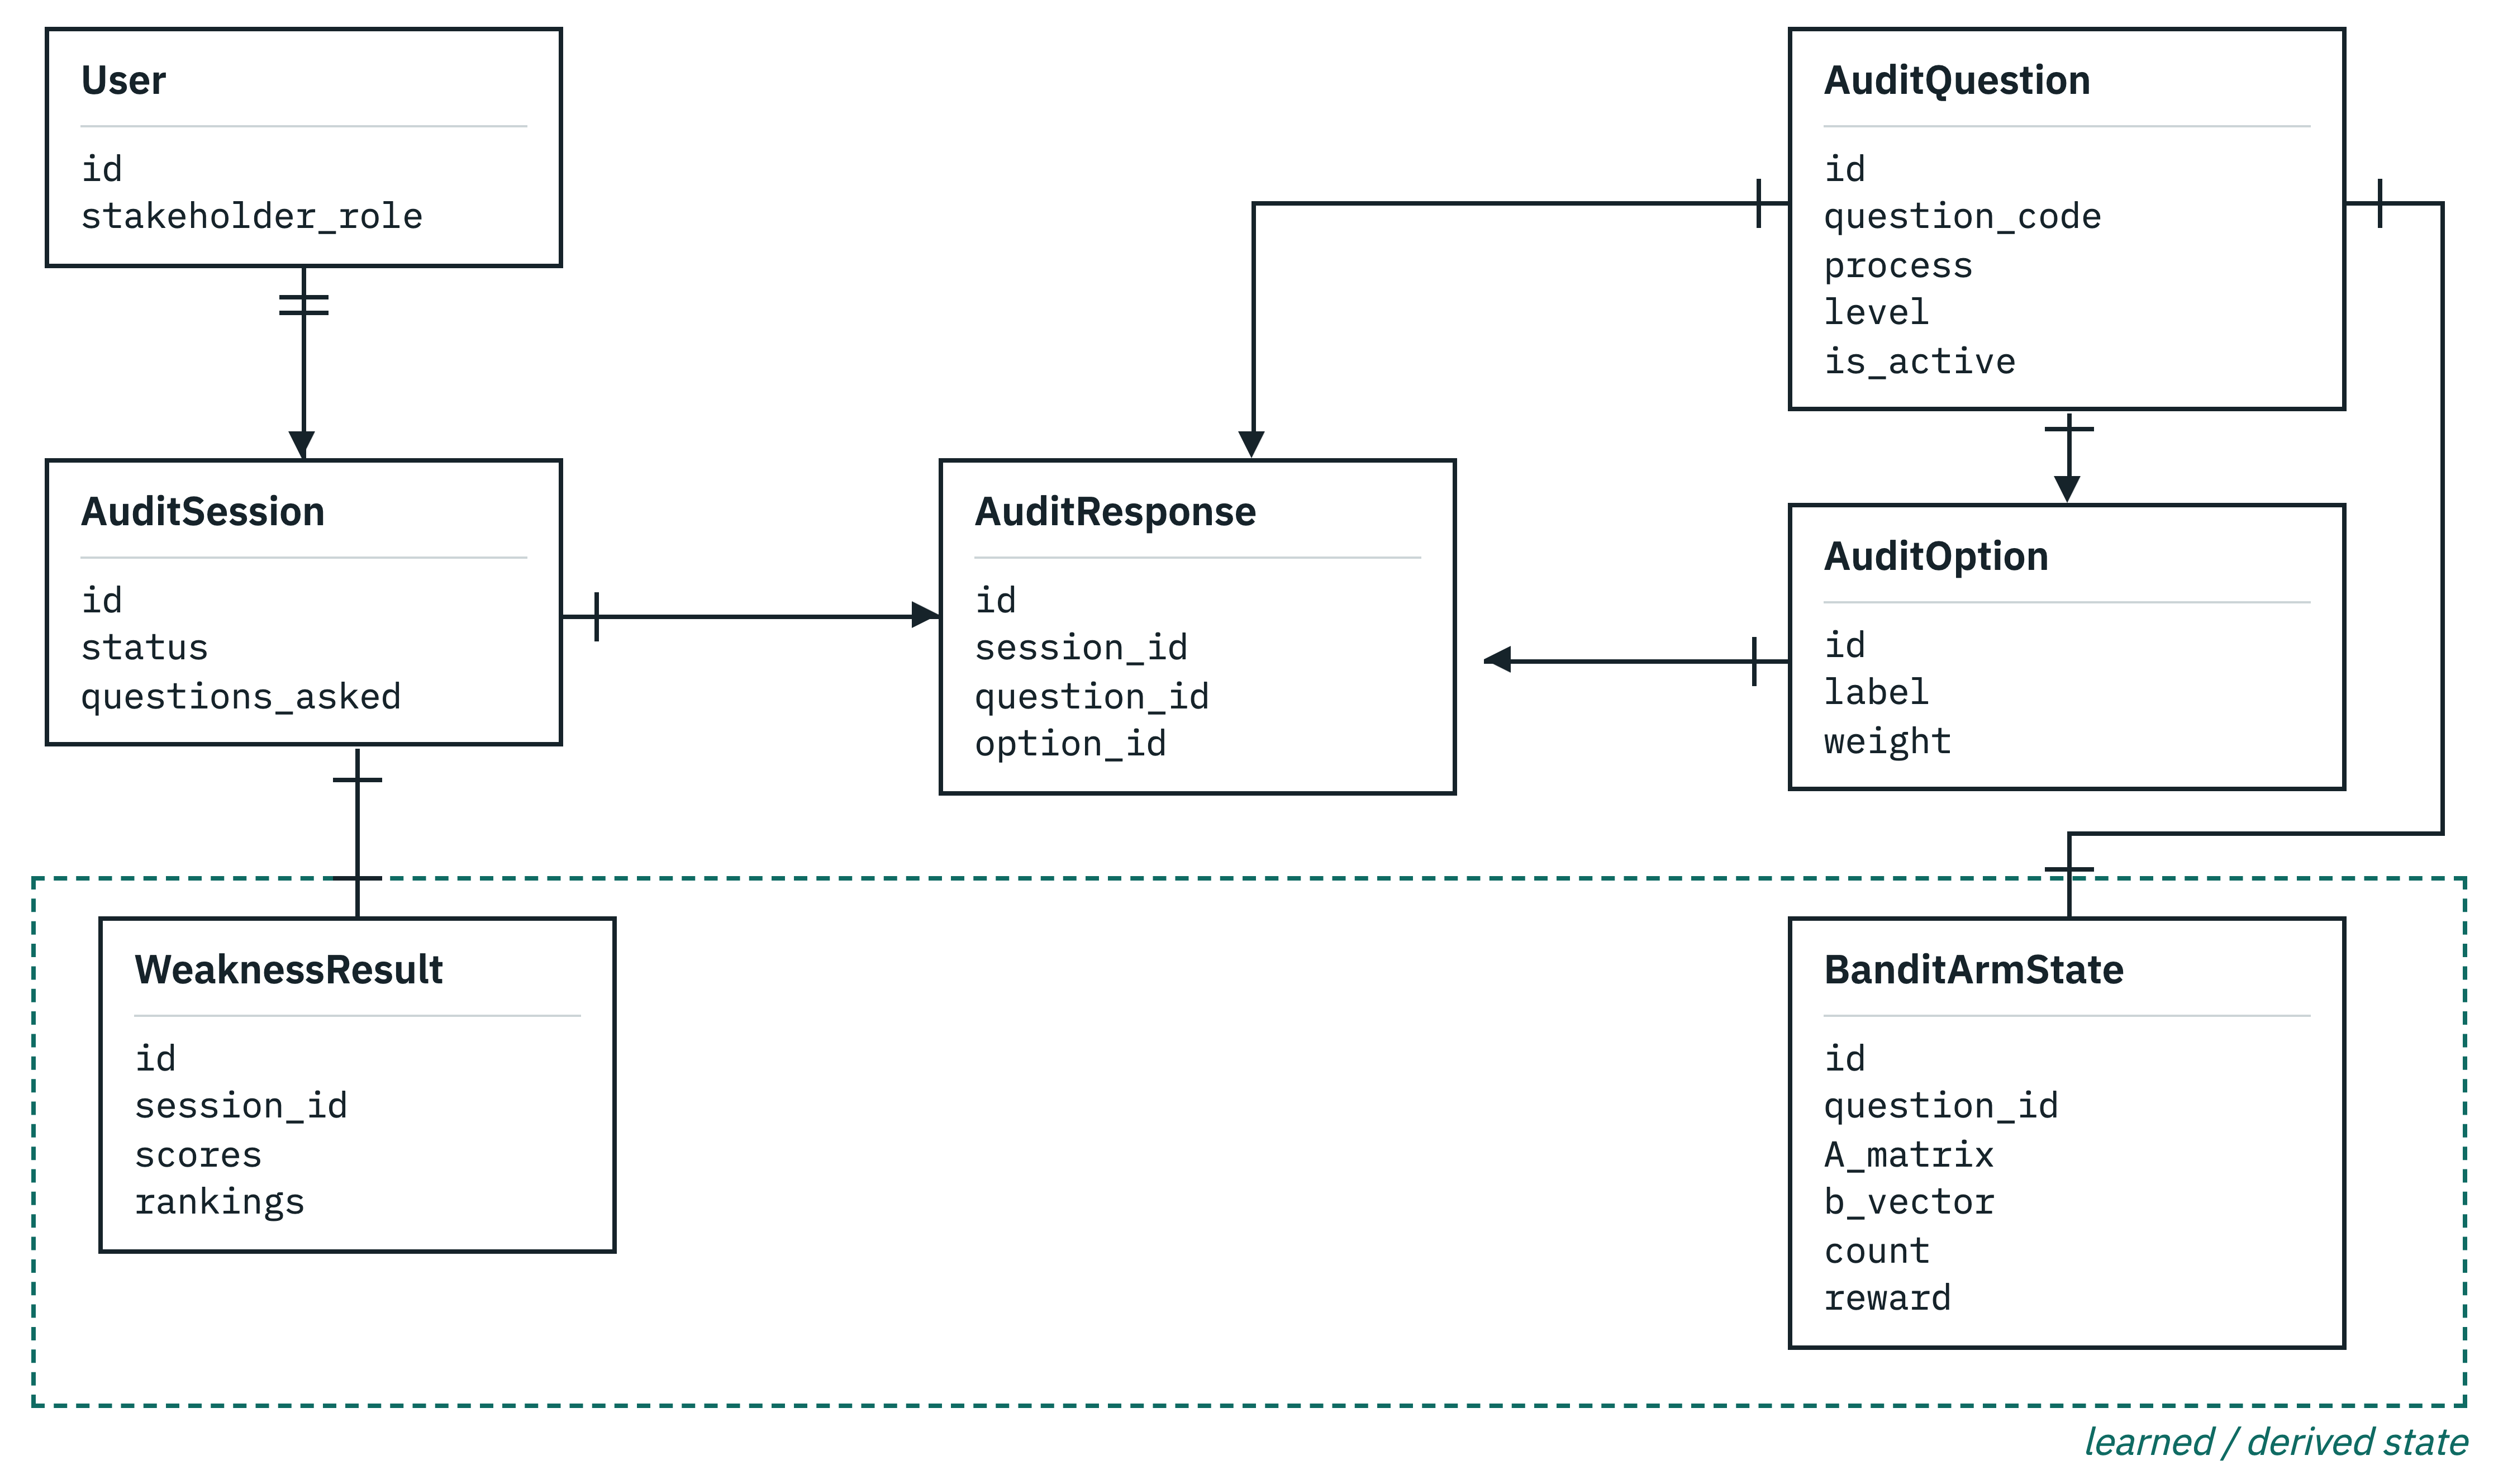
\includegraphics[width=\textwidth]{src/Arch_4.png}
  \caption{Entity-relationship diagram of the database schema.}
  \label{fig:erd}
\end{figure}

At the center of the schema is a simple chain: a \texttt{User} starts many
\texttt{AuditSession}s over time, each session collects many \texttt{AuditResponse} rows as the
stakeholder answers questions, and each response points to the specific
\texttt{AuditQuestion} that was asked and the \texttt{AuditOption} that was chosen. Two more
tables hang off the ends of that chain rather than sitting inside it. A
\texttt{WeaknessResult} belongs to exactly one completed session, it is the session's final
verdict. A \texttt{BanditArmState} belongs to exactly one question, it is that question's
running memory of how it has performed so far, independent of any single session or user. Put
plainly: sessions and responses record what happened; results and bandit state record what was
learned from it.

\subsection{User and Question Models}

The \texttt{User} table is the same one the rest of the application already relies on for login,
extended with one new field: \texttt{stakeholder\_role}, collected once at signup and never
asked again. That single field is what lets every later step, which questions are eligible,
which results a person sees, work without having to ask a stakeholder to re-identify themselves
every time.

\texttt{AuditQuestion} is the table version of everything Section~\ref{sec:answer-weighting}
walked through by hand: a \texttt{question\_code}, a \texttt{process} and \texttt{level}, the
\texttt{base\_practice\_id} that ties it back to the standard, the question text itself, the list
of stakeholder roles it is eligible for, and the recommendation shown when it is answered poorly.
One field is worth calling out specifically: \texttt{is\_active}. Questions are never deleted
outright; instead they are switched off. This matters more than it sounds, because a question
that was already answered by a real stakeholder cannot simply disappear from the database
without leaving that person's past answer pointing at nothing. \texttt{AuditOption} sits directly
underneath a question, one row per answer choice, each carrying the label, the option text, and
the weight described in Section~\ref{sec:answer-weighting}.

\subsection{Assessment Session and Response Models}

An \texttt{AuditSession} is deliberately thin. It tracks who is taking it, whether it is still
\texttt{in\_progress}, \texttt{completed}, or was \texttt{abandoned}, how many questions it is
allowed to ask before it has to stop, and the ordered list of question IDs it has already served.
That last field, \texttt{questions\_asked}, is what makes the session self-aware: every time the
system has to decide what to ask next, it already knows exactly what it asked before, without
needing to reconstruct that history from anywhere else. Each answer a stakeholder actually gives
becomes its own \texttt{AuditResponse} row: which session it belongs to, which question was
asked, which option was picked, and when. Keeping one row per answer, rather than folding
answers into the session itself, is what lets the weakness classifier later go back and group
responses however it needs to, by process, by level, by question, without the session table
having to anticipate every possible grouping in advance.

\subsection{Result and CMAB State Models}
\label{sec:result-cmab-models}

The last two tables are where the system's two forms of intelligence are stored, and they are
kept deliberately separate from each other and from everything above them.

\texttt{WeaknessResult} exists once per completed session. It holds the score computed for every
(process, level) pair that session touched, and the small ranked list of the worst ones. It is
written once, at the moment a session finishes, and never changed afterwards, it is a record of a
verdict, not a live value.

\texttt{BanditArmState} is the opposite kind of table: it exists once per question, not per
session, and it changes constantly. It holds the two matrices LinUCB needs to keep learning, a
running count of how often the question has been picked, and its cumulative reward so far. Every
stakeholder who ever answers that question, in any session, updates the same row.

Keeping \texttt{BanditArmState} out of \texttt{AuditQuestion} is a deliberate choice, not an
accident of normalization. Question content changes rarely, and only when an administrator edits
it; the bandit's learned parameters change after every single answer, from every session,
continuously. Bundling the two into one table would mean that editing a question's wording and
updating what the algorithm has learned about it become the same operation, which they are not,
and should not be.

\section{CMAB Recommendation Engine}
\label{sec:cmab-engine}

Chapter~\ref{chap:background} introduced the contextual bandit idea in the abstract: arms,
rounds, context, reward. This section grounds that abstraction in the actual objects the system
works with.

\subsection{Mapping Assessment to the CMAB Problem}

Every active \texttt{AuditQuestion} a stakeholder is allowed to see is one arm; a round is one
answered question. The engine is not learning one global ``best question,'' but, per question,
how rewarding it tends to be for a given role at a given point in a session. That per-arm state
is the \texttt{BanditArmState} row from Section~\ref{sec:result-cmab-models}: one row per
question, updated after every session that touches it and never reset.

\subsection{Context Vector}

Before scoring anything, the engine describes the situation it is in: the 23-dimensional context
vector $x$ Chapter~\ref{chap:background} referred to only in the abstract. It is rebuilt fresh
for every request, never cached: seven dimensions one-hot encode the stakeholder's role, one is
progress toward the question budget, six flag which SWE processes the session has already
touched, three flag which capability levels it has touched, and the last six carry a running
weakness score per process from the answers given so far. The role dimensions let the same
question be informative for one role and irrelevant for another; the coverage flags let the
engine notice, mid-session, that it has neglected a process, and adjust.

\subsection{Arm Eligibility}

Before scoring, the engine filters the active question bank down to admissible arms: the
question's stakeholder list must include the current user's role, and it must not already appear
in \texttt{questions\_asked} for this session. Both are hard constraints, enforced directly
rather than left for LinUCB to learn to avoid, and filtering first keeps the UCB computation
below to only the handful of questions that could plausibly be asked next.

\subsection{LinUCB Question Selection}

Selection follows the rule derived in Chapter~\ref{chap:background}: for each eligible arm $a$,
the engine computes $\theta_a = A_a^{-1} b_a$ from that arm's stored matrices, scores it as
$\mathrm{UCB}_a(x) = \theta_a^\top x + \alpha \sqrt{x^\top A_a^{-1} x}$ against the context vector
just built, and returns the arm with the highest score. The exploration coefficient $\alpha$
starts at $1.0$, a single, explainable hyperparameter revisited in Chapter~\ref{chap:results}.
Because the score is a deterministic function of $A_a$, $b_a$, and $x$, the same session history
always produces the same next question.

\subsection{Reward Function}

The base reward is the chosen option's weight, from Section~\ref{sec:answer-weighting},
normalized to $0.0$--$1.0$. A question earns a coverage bonus of $0.2$ if it is the first this
session has asked from its process, and no bonus otherwise; the two are added and clamped at
$1.0$. The bonus exists because weight alone is not a safe signal: without it, an engine chasing
weight could keep returning to one heavily-weighted process and never spend the session's limited
budget on the rest, so the bonus makes breadth pay directly.

\subsection{Online Update and State Persistence}

The reward is applied only to the arm chosen, following $A_a \leftarrow A_a + x x^\top$ and
$b_a \leftarrow b_a + r\,x$. The updated matrices are written straight back to that question's
\texttt{BanditArmState} row, so learning survives the request that produced it and is never
scoped to one session or user: every stakeholder who answers a given question, in any session,
updates the same row. A question never asked before starts from $A_a = I$ and $b_a = \mathbf{0}$.

\subsection{Session Budget}

Each \texttt{AuditSession} carries a \texttt{max\_questions} field, twelve by default and
configurable per audit. The session ends, and hands off to the weakness classifier, once
\texttt{questions\_asked} reaches that count or the eligible pool runs out. This budget is the
constraint the whole engine exists to work within: a fixed questionnaire could simply ask every
question in the bank; the point of this engine is to get as much diagnostic value as possible out
of a stakeholder who only has time for twelve.
\section{Weakness Classification and Result Generation}
\label{sec:weakness-classification}

Once a session ends, the CMAB engine's job is done and a different, much simpler piece of logic
takes over: turning a pile of answered questions into a verdict.

\subsection{Response Scoring}

Every answered question contributes one number: its option's weight, normalized to
$0.0$--$1.0$ by the same division used for the reward
(Section~\ref{sec:cmab-engine}). Because the seeded bank's weights actually run $0, 2, 3, 4, 5$
rather than stopping at $4$, a handful of individual answers normalize to just above $1.0$; this
does not break anything downstream, since the classification step in
Section~\ref{sec:classification-thresholds} treats any score past its top threshold the same way,
but it is worth naming rather than quietly rounding away.

\subsection{Process $\times$ Capability-Level Scoring}

Every response belongs to exactly one (process, level) pair, taken from the question it answers.
The classifier buckets all of a session's responses by that pair and averages the normalized
weights within each bucket, producing one score for each of the $6 \times 3 = 18$
process-level cells. A pair the session never asked about is left as \texttt{null}, not zero;
zero would claim the process was checked and found compliant, when really it was simply never
assessed in this session.

\subsection{Classification and Thresholds}
\label{sec:classification-thresholds}

Each of the 18 scores is mapped to one of four bands, shown in
Table~\ref{tab:classification-thresholds}. This is the four-band refinement of the 2024
supervisor paper's three-band traffic light, already introduced in Chapter~\ref{chap:sota}.

\begin{table}[h]
\centering
\caption{Weakness classification thresholds.}
\label{tab:classification-thresholds}
\begin{tabular}{|c|l|c|}
\hline
\textbf{Score range} & \textbf{Classification} & \textbf{Colour} \\
\hline
0.00 -- 0.25 & Compliant & Green \\
\hline
0.25 -- 0.50 & Minor Weakness & Yellow \\
\hline
0.50 -- 0.75 & Significant Gap & Orange \\
\hline
0.75 -- 1.00 & Critical Gap & Red \\
\hline
\end{tabular}
\end{table}

\subsection{Weakness Ranking}

Compliance is not the interesting part of the result; the worst gaps are. Once every assessed
cell has a score, the classifier sorts them and keeps the top three, formatted as
\texttt{"SWE3-L2"}-style keys. Cells left \texttt{null} take no part in this ranking, an
unassessed process is not, by default, treated as a weak one.

\subsection{Result Generation}

Figure~\ref{fig:question-to-result} ties this section together with
Section~\ref{sec:cmab-engine}: the top row repeats once per question, up to the session budget,
and the bottom row runs once, at session end, once that budget is reached.

\begin{figure}[h]
  \centering
  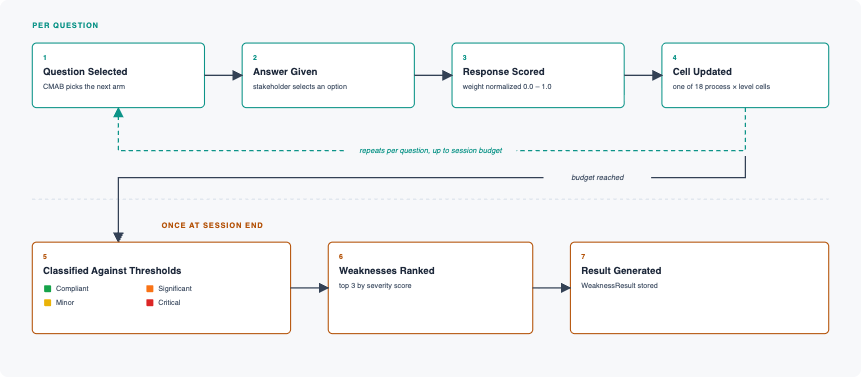
\includegraphics[width=\textwidth]{src/Arch_5.png}
  \caption{Question-to-result processing flow, from question selection to a stored result.}
  \label{fig:question-to-result}
\end{figure}

The 18 scores and the top three weaknesses are written once, together, into a single
\texttt{WeaknessResult} row for that session, alongside a timestamp. This is the same
write-once, never-updated record described in Section~\ref{sec:result-cmab-models}: a session's
final verdict, not a value that changes after the fact. It is also the last step before the
stakeholder ever sees a result, everything the results dashboard in
Section~\ref{sec:user-interface-design} displays is read directly from this one row.
\section{API and Interaction Design}
\label{sec:api-design}

Everything described so far, the question bank, the database, the CMAB engine, the classifier,
is reached from outside through one thing: a single versioned REST API.

\subsection{API Responsibilities}

The API layer is deliberately thin. Its routes authenticate a request and hand it to the
relevant service from earlier in this chapter; they contain no business logic of their own.
Every route under \texttt{/api/v1} falls into one of three groups: audit session endpoints,
usable by any authenticated stakeholder; question bank endpoints, letting an administrator
create, edit, and deactivate questions (Section~\ref{sec:answer-weighting}); and analytics
endpoints, giving an administrator aggregate views across every session, feeding the admin
interface in Section~\ref{sec:user-interface-design}.

\subsection{Authentication and Authorization}

Access is JWT-based: logging in issues a token, and every subsequent request carries it.
Signup collects a stakeholder's \texttt{stakeholder\_role} once, as described in
Section~\ref{sec:requirements-analysis}. An \texttt{is\_superuser} flag on the user account is
what separates an ordinary stakeholder from an administrator; question bank and analytics
endpoints check for it explicitly, while audit session endpoints only require a valid token.
This satisfies NFR3 from Section~\ref{sec:requirements-analysis}.

\subsection{Assessment Session Interaction}

Table~\ref{tab:session-endpoints} lists the endpoints a stakeholder uses to take part in an
assessment, before submitting any answer.

\begin{table}[h]
\centering
\caption{Assessment session endpoints.}
\label{tab:session-endpoints}
\begin{tabular}{|l|p{6.5cm}|}
\hline
\textbf{Endpoint} & \textbf{Purpose} \\
\hline
\texttt{POST /audit/sessions/} & Start a new session; returns the first selected question. \\
\hline
\texttt{GET /audit/sessions/} & List the current user's own sessions, past and present. \\
\hline
\texttt{GET /audit/sessions/\{id\}} & Retrieve one session's detail, including every question
asked so far. \\
\hline
\end{tabular}
\end{table}

\subsection{Answer Submission and Result Retrieval}

\begin{figure}[h]
  \centering
  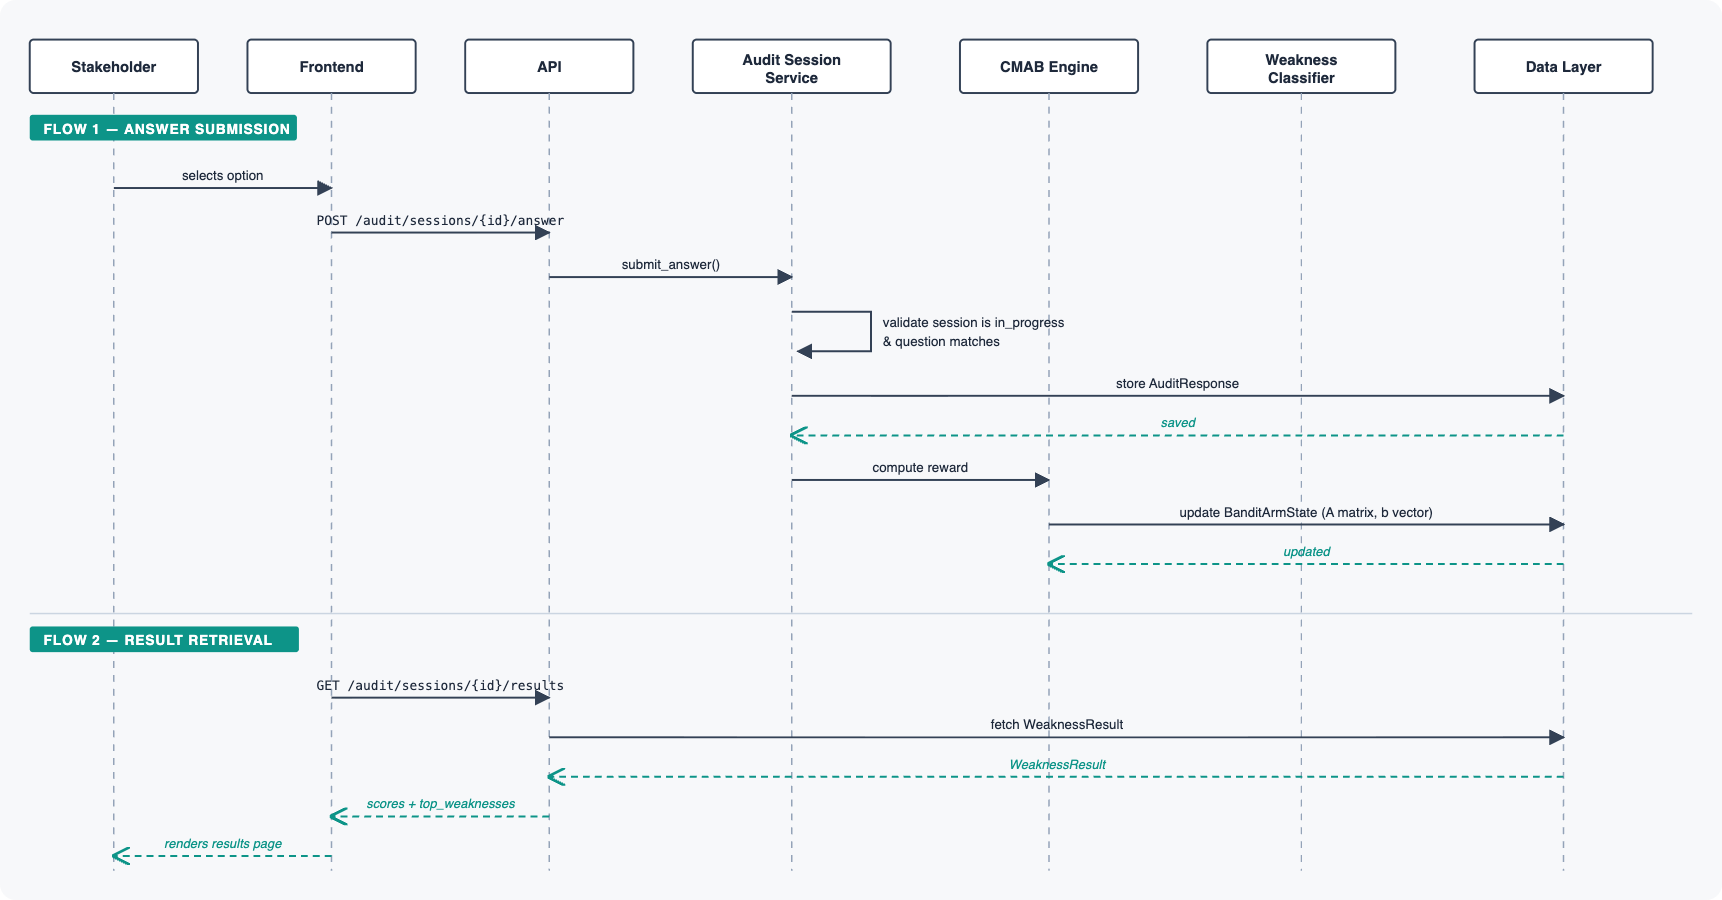
\includegraphics[width=\textwidth]{src/Arch_6_Sequence_diagram.png}
  \caption{Answer submission and result retrieval sequence.}
  \label{fig:arch-answer-sequence}
\end{figure}

Figure~\ref{fig:arch-answer-sequence} shows this interaction end to end. A single answer-submission
endpoint carries almost the entire interaction described in Sections~\ref{sec:cmab-engine}
and~\ref{sec:weakness-classification}.
It validates that the session is still in progress and that the answered question is really the
one the session was waiting on, stores the response, computes its reward, and updates the
answered question's \texttt{BanditArmState}. From there it branches: if the session's question
budget has not been reached, it selects and returns the next question; otherwise it runs the
classifier, stores the resulting \texttt{WeaknessResult}, and marks the session completed. A
separate results endpoint retrieves that stored result once
it exists. Splitting the two matters for the frontend: a session can be polled for its result
independently of the request that produced it, so nothing about the result depends on the client
still being connected at the moment the session finished.

\section{User Interface Design}
\label{sec:user-interface-design}

The interface is where every design decision so far becomes something a stakeholder actually
sees and clicks through, so it is organized around the same role split as the API.

\subsection{User Roles and Views}

There are two kinds of user, and each sees a different set of views. Any authenticated
stakeholder sees the views that make up an assessment: starting and taking a session, seeing its
results, and browsing their own session history. An administrator, distinguished by the same
\texttt{is\_superuser} flag checked at the API level (Section~\ref{sec:api-design}), additionally
sees the question bank manager and the analytics dashboard; nothing about the assessment views
themselves changes for an administrator, they simply have extra views layered on top.

\subsection{Assessment Session Flow}

Starting a session immediately returns its first question, so a stakeholder never sees an empty
screen. Questions are shown one at a time, with their five options and a progress indicator
(``Question 3 of 12''), matching the one-question-at-a-time interaction already described in
Section~\ref{sec:api-design}. Submitting an answer does one of two things: it replaces the
current question with whatever the CMAB engine selects next, or, once the session's budget is
reached, it moves the stakeholder straight to their results. Signup asks for a stakeholder's role
exactly once, the same field described in Section~\ref{sec:requirements-analysis}, and never
again afterward.

\subsection{Results Visualization}

A finished session's \texttt{WeaknessResult} (Section~\ref{sec:weakness-classification}) is
presented three ways, each answering a different question. A radar chart, one axis per SWE
process, gives an at-a-glance shape of overall process health. A heatmap table, processes against
capability levels, colour-codes every assessed cell by the same four bands from
Table~\ref{tab:classification-thresholds}, so a stakeholder can see exactly where, not just how
badly, a weakness sits. A ranked list of the top three weaknesses pairs each one with the
recommendation text carried by the question that exposed it, so the result ends in something
actionable, not just a score.

\subsection{Administration Interface}

Administrators see two additional views, matching the two admin-only endpoint groups from
Section~\ref{sec:api-design}. The question bank manager lists, filters, and edits questions and
their options directly, giving administrators create/edit/deactivate control over the question
bank maintained under FR3 (Section~\ref{sec:requirements-analysis}). The analytics dashboard aggregates across every
completed session at once: a weakness heatmap covering the whole question bank rather than one
session, CMAB arm statistics showing which questions are pulled most often and how rewarding they
have been, and participation counts by stakeholder role. Where the stakeholder-facing views
answer ``how did this session go,'' this view answers ``how is the system behaving overall.''

\section{Key Design Decisions and Trade-offs}
\subsection{LinUCB versus Alternative Algorithms}

Chapter~\ref{chap:background} introduced four ways to handle the exploration--exploitation
trade-off: Epoch-Greedy, $\epsilon$-greedy, Thompson Sampling, and UCB-style methods, of which
LinUCB is the contextual member this thesis actually uses. This subsection makes that choice
explicit, and confronts the one piece of evidence that argues against it.

That evidence is not hidden: Chapter~\ref{chap:sota}'s Table~\ref{tab:recommender-results},
reproduced from the closest prior work, shows $\epsilon$-greedy beating LinUCB on raw reward in
every simulated scenario tested, by roughly 13 percentage points at a 0\% deficiency-change rate,
narrowing to about 1 point at 50\%~\cite{datsogiannis2025recommender}. So this is not a choice
made because LinUCB is known to score highest; it is a choice made for what a thesis evaluation
actually needs, which is not quite the same thing as raw average reward.

Table~\ref{tab:algorithm-comparison} lays out the four candidates against the properties that
matter here.

\begin{table}[h]
\centering
\caption{Bandit algorithms considered, compared on the properties relevant to this thesis.}
\label{tab:algorithm-comparison}
\begin{tabular}{|l|p{4.3cm}|c|c|}
\hline
\textbf{Algorithm} & \textbf{Selection rule} & \textbf{Deterministic?} & \textbf{Context-aware?} \\
\hline
Epoch-Greedy~\cite{langford2007epochgreedy} & Alternates fixed explore/exploit
blocks & Within a block & No \\
\hline
$\epsilon$-greedy~\cite{tokic2011valuedifference} & Best known arm, or a
random arm with probability $\epsilon$ & No & No \\
\hline
Thompson Sampling~\cite{agrawal2013thompson} & Samples an arm from a fitted
reward distribution & No & Contextual only \\
\hline
LinUCB~\cite{li2010contextual,huang2016linucb} & $\theta_a^\top x + \alpha
\sqrt{x^\top A_a^{-1} x}$, highest score wins & Yes & Yes, natively \\
\hline
\end{tabular}
\end{table}

Three reasons, all visible in that table, decided the choice. First, \textbf{determinism}. Both
$\epsilon$-greedy and Thompson Sampling select by drawing a random number on every single round,
either to decide whether to explore at all, or to sample directly from a posterior. That is a
reasonable design for a production system averaging behavior over millions of rounds, but it is
an awkward one for a thesis: the same context and the same model state can legitimately produce
a different next question on a different run, which makes any single session's selections hard
to walk through and defend after the fact. LinUCB's score is a deterministic function of $A_a$,
$b_a$, and $x$ alone, so a specific session's specific sequence of questions can always be
recomputed and explained, not just observed.

Second, \textbf{native context-awareness}. Plain $\epsilon$-greedy and plain UCB score an arm
only from its own historical average reward; they have no way to express that a question matters
for a QA Engineer but not a Project Manager, or that it matters more three questions into a
session than at the start, without a separate mechanism bolted on top. LinUCB's whole scoring
rule is built around the 23-dimensional context vector from Section~\ref{sec:cmab-engine}: the
$\theta_a^\top x$ term is not an addition to the algorithm, it is the algorithm. Thompson
Sampling has contextual variants, but the version benchmarked in
Table~\ref{tab:recommender-results} was not one of them.

Third, \textbf{one explainable hyperparameter}. LinUCB's exploration coefficient $\alpha$ has a
direct, statable meaning: how much weight the uncertainty bonus gets relative to the plain reward
estimate. $\epsilon$-greedy's exploration is cruder by comparison, a fixed or decaying
probability of ignoring context entirely, and Thompson Sampling's exploration is implicit in a
fitted distribution that is harder to describe to a reader without a Bayesian background.

None of this makes $\epsilon$-greedy's simulated result irrelevant. It is a real number, from the
closest prior work, and it says LinUCB is not the best-scoring option under pure reward
maximization on simulated data. What it does not settle is whether that gap holds up on real,
non-simulated pilot sessions, the one evaluation neither prior paper ran. Whether it does is an
empirical question this thesis is positioned to actually answer, and
Chapter~\ref{chap:results} returns to it directly.

\subsection{Adaptive versus Static Questionnaire}
\subsection{Weight-Based Reward versus Expert Labels}
\subsection{Rule-Based versus ML-Based Classification}

\section{Chapter Summary}

This chapter turned the requirements from Section~\ref{sec:requirements-analysis} into a
concrete design: an overall architecture built around a CMAB engine and a weakness classifier
sitting on top of a shared database, a question bank that ties every question back to a specific
ASPICE base practice, and a REST API and user interface that expose the whole thing to
stakeholders and administrators without leaking any of that internal structure to them. Where a
design decision had a real alternative, this chapter named it and argued for the choice actually
made, most visibly the decision to use LinUCB despite prior evidence that a simpler algorithm
scores higher in simulation. Chapter~\ref{chap:implementation} now turns this design into running
code.

\chapter{Implementation (12--14 pages)}
\label{chap:implementation}
% \input{src/implementation}
\section{Development Environment and Tooling}
\subsection{Containerized Development Environment (Docker Compose Watch)}
\subsection{Backend Development Stack (FastAPI, SQLModel, uv, Alembic)}
\subsection{Frontend Development Stack (React, TypeScript, Vite, TanStack Router)}
\section{Backend Implementation}
\subsection{Backend Project Structure}
\subsection{Data Models and Database Migrations}
\subsection{Audit Session Service (\texttt{audit\_service.py})}
\subsection{CMAB Engine Implementation (\texttt{cmab\_engine.py})}
\subsection{Weakness Classifier Implementation (\texttt{weakness\_classifier.py})}
\subsection{API Routes and Dependency Injection}
\subsection{Authentication and Authorization}
\section{Question Bank Implementation}
\subsection{Question Bank Data Preparation}
\subsection{Seed Script and Idempotent Seeding}
\subsection{Traceability and Stakeholder Role Fields}
\section{Frontend Implementation}
\subsection{Frontend Project Structure and Routing}
\subsection{Authentication and User Management}
\subsection{Assessment Session and Question Interaction (Screenshots)}
\subsection{Results Dashboard and Visualization (Screenshots)}
\subsection{Administration and Question Bank Management (Screenshots)}
\section{Deployment and Runtime Configuration}
\subsection{Docker Compose Services, Networking, and Volumes}
\subsection{Traefik Reverse Proxy, HTTPS, and Production Deployment}
\subsection{Environment Configuration and Secrets}
\section{Implementation Challenges and Solutions}
\subsection{CMAB State Persistence}
\subsection{Maintaining Question Selection Constraints}
\subsection{Synchronization Between Session State and Database}
\subsection{Frontend--Backend Integration Issues}
\section{Chapter Summary}

\chapter{Evaluation Methodology (49--58 pages)}
\label{chap:methodology}
% \input{src/methodology}
\section{Evaluation Goals Revisited}
\section{Software Quality Verification}
\subsection{Unit Testing Strategy (pytest, Service-Level Tests)}
\subsection{Test Coverage Summary}
\section{Functional and Smoke Testing of the Application}
\subsection{Test Case Design (Signup $\to$ Session $\to$ Answer $\to$ Results)}
\subsection{Health Check and Environment Verification}
\section{Pilot Usage Sessions}
\subsection{Participants and Stakeholder Roles Represented}
\subsection{Session Protocol (Number of Sessions, Question Budget)}
\subsection{Data Collected via Existing Analytics Endpoints}
\section{Metrics Derived from Real Usage}
\subsection{CMAB Arm Statistics (Pull Count, Average Reward)}
\subsection{Weakness Score Distributions}
\section{Chapter Summary}

\chapter{Results and Evaluation (59--73 pages)}
\label{chap:results}
% \input{src/results}
\section{Software Quality Assurance Results}
\subsection{Unit Test Outcomes}
\subsection{Static Analysis / Linting Outcomes}
\section{Functional Verification Results}
\subsection{End-to-End Flow Walkthrough (Screenshots)}
\subsection{Smoke Test Outcomes}
\section{CMAB Behaviour Observed from Real Pilot Sessions}
\subsection{Question Selection Patterns per Stakeholder Role}
\subsection{Bandit Arm Statistics (Real Pull Counts and Rewards)}
\subsection{Process Coverage Achieved within the 12-Question Budget}
\section{Weakness Classification Results from Pilot Sessions}
\subsection{Individual Session Heatmaps and Radar Charts}
\subsection{Aggregate Weakness Heatmap across All Pilot Sessions}
\section{System Performance}
\subsection{API Response Latency}
\subsection{Session Completion Time vs.\ Manual Assessment Duration}
\section{Discussion of Results}
\section{Threats to Validity}
\section{Chapter Summary}

\chapter{Conclusion and Future Work (74--80 pages)}
\label{chap:conclusion}
% \input{src/conclusion}
\section{Summary of Contributions}
\section{Answering the Research Questions}
\section{Limitations}
\section{Future Work}
\subsection{Larger-Scale Pilot with Certified ASPICE Assessors}
\subsection{Simulation-Based Benchmarking of LinUCB against Baselines}
\subsection{Supervised Weakness Classifier from Accumulated Sessions}
\subsection{Expert/Assessor-Validated Reward Signal}
\subsection{Expansion to Additional ASPICE Process Groups (SYS, MAN, SUP)}
\section{Final Remarks}

%---------------------------------------------------------
% bibliography based on Springer Design
%---------------------------------------------------------

\bibliographystyle{splncs03}
\bibliography{bibliography}

%---------------------------------------------------------
% Appendices
%---------------------------------------------------------

\appendix
\chapter{ASPICE Question Bank}
\label{app:questionbank}
Full list of the 42 questions and 210 options used in the seeded question bank, covering SWE.1--SWE.6.

\chapter{Database Schema}
\label{app:dbschema}
Full DDL and entity-relationship diagram.

\chapter{API Reference}
\label{app:apiref}
OpenAPI specification excerpt.

\chapter{Pilot Session Raw Data}
\label{app:pilotdata}
Raw exports from the \texttt{/analytics/bandit} and \texttt{/analytics/weaknesses} endpoints.

\chapter{Additional Screenshots}
\label{app:screenshots}
Admin dashboard, history page, and signup flow.

\chapter{Deployment Configuration Files}
\label{app:deployment}
Docker Compose and Traefik configuration listings.

\printindex

\end{document}
